\section{Affiliated and Asymmetric Private Values}\label{sec:15-apv}

The inversion of \cref{sec:15-gpv} rests on two assumptions besides private values. Values are
independent across bidders, and bidders are symmetric. Both assumptions often fail. Bidders who appraise
the same tract of timber tend to have correlated values. They react to features of the tract that the
econometrician does not record. Bidders also differ in systematic ways. A sawmill differs from a logger,
a consortium from a single firm, and a contractor next to the site from one far away.

This section shows that the first-order condition can still be inverted when both assumptions fail. The
key observable becomes the joint distribution of a bidder's own bid and the highest rival bid. We first
treat symmetric affiliated private values \citep{LiPerrigneVuong2002}. We then ask what the two highest
bids alone reveal \citep{AtheyHaile2002}. Next we study asymmetric affiliated private values and joint
bidding for offshore oil leases \citep{CampoPerrigneVuong2003}. We close with asymmetric independent
private values.

\subsection{Symmetric affiliated private values: Li, Perrigne and Vuong (2002)}\label{sec:15-apv-lpv}

\casehead{Question} Before 2002, structural work on first-price auctions used either the independent
private value (IPV) model or the pure common value model. \citet{LiPerrigneVuong2002}, henceforth LPV, ask whether the
\emph{affiliated private value} (APV) model can be identified and estimated from bids alone, without a
parametric form for the dependence among values. The question matters because affiliation changes
equilibrium shading. An analyst who imposes independence on affiliated data misreads bids, and so
misreads values and rents.

\casehead{Model} A single object is sold by first-price sealed bid to $n\ge2$ risk-neutral bidders. In the
affiliated value model of \citet{MilgromWeber1982}, bidder $i$'s utility is $U(v_i,c)$, where $v_i$ is
her private signal and $c$ a common component. The APV model is the case $U(v,c)=v$. Values
$\bm V=(V_1,\dots,V_n)$ have a joint distribution $F$ with density $f$ on $[\underline v,\bar v]^n$. The
density is symmetric (exchangeable) and affiliated in the sense of \cref{def:14-affiliation}. The reserve
price does not bind. Let $Y_1=\max_{j\ne1}V_j$ be the highest rival value. Write $F_{Y_1\mid V_1}$ and
$f_{Y_1\mid V_1}$ for its conditional distribution and density given $V_1$. Affiliation leaves the form of
dependence unrestricted. A common component plus independent noise is one example among many.

The symmetric equilibrium in strictly increasing strategies $\beta$ is the special case of
\cref{prop:14-mw-fpa} with $v(\alpha,\alpha)=\alpha$. It solves the differential equation
\begin{equation}\label{eq:15-lpv-ode}
  \beta'(v)=\bigl(v-\beta(v)\bigr)\frac{f_{Y_1\mid V_1}(v\mid v)}{F_{Y_1\mid V_1}(v\mid v)},
  \qquad \beta(\underline v)=\underline v,
\end{equation}
which is equation (1) of \citet{LiPerrigneVuong2002}. Its solution is
\begin{equation}\label{eq:15-lpv-bid}
  \beta(v)=v-\int_{\underline v}^{v}L(\alpha\mid v)\,d\alpha,
  \qquad
  L(\alpha\mid v)=\exp\left(-\int_\alpha^v\frac{f_{Y_1\mid V_1}(u\mid u)}{F_{Y_1\mid V_1}(u\mid u)}\,du\right),
\end{equation}
their equation (2). The bid depends on $F$ through the whole conditional law of the highest rival value
along the diagonal. A parametric family for $F$, such as a multivariate lognormal, rarely yields a closed
form for $\beta$.

\casehead{From the differential equation to observables} Bids are random with joint distribution
$\bm G$, which the econometrician observes when all bids are recorded. Let $B_i$ be bidder $i$'s bid and
$M_i=\max_{j\ne i}B_j$ the highest rival bid. Let $G_{M\mid B}(m\mid b)=\Pr(M_i\le m\mid B_i=b)$, with
density $g_{M\mid B}(m\mid b)$ in $m$. Because $\beta$ is strictly increasing, $M_1=\beta(Y_1)$ and the
event $\{B_1=b\}$ equals $\{V_1=\beta^{-1}(b)\}$. Hence
\begin{align*}
  G_{M\mid B}(m\mid b)&=\Pr\bigl(\beta(Y_1)\le m\mid \beta(V_1)=b\bigr)
  =F_{Y_1\mid V_1}\bigl(\beta^{-1}(m)\mid\beta^{-1}(b)\bigr),\\
  g_{M\mid B}(m\mid b)&=\frac{f_{Y_1\mid V_1}\bigl(\beta^{-1}(m)\mid\beta^{-1}(b)\bigr)}{\beta'\bigl(\beta^{-1}(m)\bigr)}.
\end{align*}
Evaluate both at $m=b=\beta(v)$ and take the ratio:
\begin{equation*}
  \frac{G_{M\mid B}(b\mid b)}{g_{M\mid B}(b\mid b)}
  =\beta'(v)\,\frac{F_{Y_1\mid V_1}(v\mid v)}{f_{Y_1\mid V_1}(v\mid v)}
  =v-\beta(v),
\end{equation*}
where the second equality is \eqref{eq:15-lpv-ode}. Rearranging gives the inverse bid function
\begin{equation}\label{eq:15-lpv-foc}
  v=\xi(b;\bm G)\equiv b+\frac{G_{M\mid B}(b\mid b)}{g_{M\mid B}(b\mid b)},
\end{equation}
equation (4) of \citet{LiPerrigneVuong2002}. It is the first-order condition \eqref{eq:14-apv-foc}
written in observables. Conditioning on the value is the same as conditioning on the bid, because the
equilibrium is strictly monotone. With independent values $G_{M\mid B}(b\mid b)=G(b)^{n-1}$, and
\eqref{eq:15-lpv-foc} reduces to the inversion \eqref{eq:15-gpv-xi}.

\begin{definition}[Rationalization in the APV model]\label{def:15-lpv-rational}
A joint distribution $\bm G$ of bids is \emph{rationalized} by an APV structure $F$ if $\bm G$ is the
equilibrium bid distribution of the first-price auction with values drawn from $F$. The APV model is
identified if no two distinct structures $F\ne\tilde F$ lead to the same $\bm G$
\citep[Definition~1]{LiPerrigneVuong2002}.
\end{definition}

\begin{proposition}[{\citealp[Proposition~1]{LiPerrigneVuong2002}}]\label{prop:15-lpv}
The symmetric APV model is identified. Let $\bm G$ have support $[\underline b,\bar b]^n$. It can be
rationalized by a symmetric APV model if and only if two conditions hold.
\begin{enumerate}[label=(\roman*)]
  \item $\bm G$ is symmetric and affiliated.
  \item $\xi(\cdot;\bm G)$ in \eqref{eq:15-lpv-foc} is strictly increasing on $[\underline b,\bar b]$.
\end{enumerate}
The sufficiency direction also maintains the boundary condition
$\frac{G_{M\mid B}(b\mid b)}{g_{M\mid B}(b\mid b)}\to0$ as $b\downarrow\underline b$, which every rationalizable $\bm G$
satisfies. The rationalizing distribution is
\begin{equation}\label{eq:15-lpv-F}
  F(v_1,\dots,v_n)=\bm G\bigl(\xi^{-1}(v_1;\bm G),\dots,\xi^{-1}(v_n;\bm G)\bigr).
\end{equation}
\end{proposition}

\begin{proof}
\emph{Identification.} Let $F$ and $\tilde F$ both generate $\bm G$, with equilibrium strategies $\beta$ and
$\tilde\beta$. Both strategies satisfy \eqref{eq:15-lpv-ode}, which is equivalent to
\eqref{eq:15-lpv-foc}. So $\beta^{-1}=\tilde\beta^{-1}=\xi(\cdot;\bm G)$, and
$F(\bm v)=\Pr\bigl(\xi(B_i)\le v_i\ \forall i\bigr)=\tilde F(\bm v)$.

\emph{Necessity.} If $F$ rationalizes $\bm G$, then $\bm G(\bm b)=F\bigl(\beta^{-1}(b_1),\dots,\beta^{-1}(b_n)\bigr)$.
Strictly increasing transformations preserve symmetry and affiliation, which gives (i). Since
$\xi=\beta^{-1}$, (ii) holds. The ratio in the boundary condition equals $\xi(b)-b=\beta^{-1}(b)-b$, which tends to
zero as $b\downarrow\underline b$ because $\beta(\underline v)=\underline v$.

\emph{Sufficiency.} Let $\bm G$ satisfy (i) and (ii) and define $F$ by \eqref{eq:15-lpv-F}. Then $F$ is a
symmetric affiliated distribution on $[\underline v,\bar v]^n$ with
$\underline v=\xi(\underline b)$ and $\bar v=\xi(\bar b)$. Let bidders use $\beta=\xi^{-1}$. Then
$\bm G=F\circ\beta^{-1}$ by construction, and the steps above reverse to show that $\beta$ solves
\eqref{eq:15-lpv-ode}. For the boundary condition, LPV argue that $\ln G_{M\mid B}$ diverges at
$\underline b$. Divergence of the logarithm alone does not force the markdown
$\frac{G_{M\mid B}(b\mid b)}{g_{M\mid B}(b\mid b)}$ to vanish. This is why the proposition maintains
that this ratio tends to zero as $b\downarrow\underline b$. A bid density bounded away from zero at $\underline b$ is
sufficient but too strong. With i.i.d.\ uniform values and $n\ge3$ the density tends to zero, yet the ratio
equals $\frac{b}{n-1}$ and still vanishes. Under the maintained condition, $\xi(\underline b)=\underline b$, so
$\beta(\underline v)=\underline v$.
Second-order conditions are maintained throughout \citep[footnote~7]{LiPerrigneVuong2002}.
\end{proof}

Three remarks place the result. First, \citet{LaffontVuong1996} show that the general affiliated value
model is not identified from bids. Any affiliated value model with fixed $n$ is observationally equivalent
to some APV model. Restricting attention to APV therefore loses nothing in explaining bids. In this
sense the symmetric APV model is the most general model identified from bids alone
\citep[p.~175]{LiPerrigneVuong2002}. It does not exclude common values. It only cannot distinguish them
(\cref{sec:15-cv-limits}). Second, condition (ii) is a testable restriction of equilibrium play, as in
\cref{thm:15-gpv-ident}. Third, condition (i) implies that independence of values can be tested through
independence of bids within auctions, for example with the test of \citet{BlumKieferRosenblatt1961}.

\casehead{Estimator} The ratio in \eqref{eq:15-lpv-foc} can be written with joint objects that are easier to
estimate. Let $G_{M,B}(m,b)=G_{M\mid B}(m\mid b)\,g_B(b)$, which is $\frac{\partial}{\partial b}\Pr(M\le
m,\,B\le b)$, and let $g_{M,B}(m,b)=g_{M\mid B}(m\mid b)\,g_B(b)$ be the joint density of $(M,B)$. Then
\begin{equation*}
  \frac{G_{M\mid B}(b\mid b)}{g_{M\mid B}(b\mid b)}
  =\frac{G_{M\mid B}(b\mid b)\,g_B(b)}{g_{M\mid B}(b\mid b)\,g_B(b)}
  =\frac{G_{M,B}(b,b)}{g_{M,B}(b,b)},
\end{equation*}
because the marginal density $g_B$ cancels. Fix $n$ and let $T_n$ be the number of $n$-bidder auctions.
With a kernel $\mathcal K$ and bandwidths $h_G$ and $h_g$, the first step computes
\begin{align}
  \hat G_{M,B}(b,b)&=\frac{1}{nT_nh_G}\sum_{t=1}^{T_n}\sum_{i=1}^{n}\indic(M_{it}\le b)\,
  \mathcal K\left(\frac{b-B_{it}}{h_G}\right),\label{eq:15-lpv-Ghat}\\
  \hat g_{M,B}(b,b)&=\frac{1}{nT_nh_g^2}\sum_{t=1}^{T_n}\sum_{i=1}^{n}
  \mathcal K\left(\frac{b-M_{it}}{h_g}\right)\mathcal K\left(\frac{b-B_{it}}{h_g}\right),\label{eq:15-lpv-ghat}
\end{align}
equations (5)--(6) of \citet{LiPerrigneVuong2002} and (3.3)--(3.4) of \citet{AtheyHaile2007}. Averaging over
the $n$ bidders in each auction uses symmetry. The pseudo-values are
\begin{equation}\label{eq:15-lpv-pseudo}
  \hat V_{it}=B_{it}+\frac{\hat G_{M,B}(B_{it},B_{it})}{\hat g_{M,B}(B_{it},B_{it})}
  \quad\text{if } B_{\min}+h_g\le B_{it}\le B_{\max}-h_g,
\end{equation}
and $\hat V_{it}=+\infty$ otherwise. Trimming bids within one bandwidth of the boundaries removes the
pseudo-values that kernel boundary bias would distort \citep[p.~181]{LiPerrigneVuong2002}.

The second step estimates the $n$-variate density of values from the auctions that survive trimming,
\begin{equation}\label{eq:15-lpv-fhat}
  \hat f(v_1,\dots,v_n)=\frac{1}{T_nh_f^n}\sum_{t=1}^{T_n}
  \mathcal K_f\left(\frac{v_1-\hat V_{1t}}{h_f},\dots,\frac{v_n-\hat V_{nt}}{h_f}\right),
\end{equation}
with a product kernel $\mathcal K_f$. A kernel with compact support gives zero weight to any auction with
an infinite pseudo-value, so trimmed auctions drop out. Symmetry is imposed by averaging $\hat f$ over the
$n!$ permutations of its arguments. The marginal density of values uses all pseudo-values,
$\hat f_n(v)=\frac{1}{nT_nh_m}\sum_t\sum_i\mathcal K\bigl(\frac{v-\hat V_{it}}{h_m}\bigr)$. Comparing
$\hat f_n$ across $n$ checks whether the value distribution depends on the number of bidders. If it does
not, pseudo-values from different $n$ can be pooled.

\begin{remark}[Rates]\label{rem:15-lpv-rates}
Let $f$ have $R$ continuous bounded derivatives. With $h_G\propto(\frac{\log T_n}{T_n})^{\frac{1}{2R+2n-3}}$,
$h_g\propto(\frac{\log T_n}{T_n})^{\frac{1}{2R+2n-2}}$ and
$h_f\propto(\frac{\log T_n}{T_n})^{\frac{R+n-2}{(R+n+1)(2R+2n-2)}}$, and if $R>n-2$, $\hat f$ is uniformly
consistent on inner compact sets with rate $(\frac{T_n}{\log T_n})^{\frac{R(R+n-2)}{(R+n+1)(2R+2n-2)}}$
\citep[Proposition~2]{LiPerrigneVuong2002}. With observed values the optimal rate would be
$(\frac{T_n}{\log T_n})^{\frac{R}{2R+n}}$ \citep{Stone1982}. For $R=2$ and $n=2$ the exponents are
$\frac{2}{15}$ and $\frac{5}{15}$. The marginal density $\hat f_n$ converges faster, with exponent
$\frac{(R+n-1)(R+n-2)}{(R+n+1)(2R+2n-2)}$ \citep[Proposition~3]{LiPerrigneVuong2002}, which equals
$\frac15$ for $R=2$ and $n=2$. Optimality of these rates is not established, because the minimax argument of
\citet{GuerrePerrigneVuong2000} does not carry over. The exponents fall with $n$. This is the curse of
dimensionality.
\end{remark}

\casehead{Implementation} \citet[pp.~180--181]{LiPerrigneVuong2002} use the triweight kernel
$\mathcal K(u)=\frac{35}{32}(1-u^2)^3\indic(|u|\le1)$, a kernel of order two, and product kernels in several
dimensions. Kernels of order three would be required in theory for $n=3$. They would produce negative
density estimates and pseudo-values below bids, so order two is used throughout. Bandwidths follow the
rate in \cref{rem:15-lpv-rates} with $R=2$. For $n=2$ they set $h_G=c_G(nT)^{-\frac15}$ and
$h_g=c_g(nT)^{-\frac16}$. For $n=3$ the exponents are $-\frac17$ and $-\frac18$. The constants follow
Silverman's rule of thumb, $c=2.978\times1.06\,\hat\sigma_b$, where $\hat\sigma_b$ is the standard
deviation of bids. The factor $2.978$ converts the rule from a Gaussian to a triweight kernel. In the second
step $h_f=c_f(2!\,T^\ast)^{-\frac{1}{15}}$ for $n=2$ and $c_f(3!\,T^\ast)^{-\frac{1}{16}}$ for $n=3$, with
$T^\ast$ the number of auctions left after trimming. When bids are skewed, the authors suggest working with
$\ln(1+b)$ and transforming back \citep[footnote~13]{LiPerrigneVuong2002}.

\casehead{Monte Carlo design} The design follows the laboratory experiments of
\citet{KagelHarstadLevin1987}. Each value is a common draw plus noise, $V_i=Q+E_i$, with $Q$ uniform on
$[\frac14,\frac34]$ and $E_i$ independent and uniform on $[-\frac14,\frac14]$. Values lie in $[0,1]$. Since
$\Var(Q)=\Var(E_i)=\frac{1}{48}$, the correlation between two values is
\begin{equation*}
  \Corr(V_i,V_j)=\frac{\Var(Q)}{\Var(Q)+\Var(E_i)}=\frac12 .
\end{equation*}
The sum of two independent uniforms of width $\frac12$ has the triangular marginal density
$f(v)=4v$ on $[0,\frac12]$ and $f(v)=4-4v$ on $[\frac12,1]$. Its kink at $\frac12$ makes it
nondifferentiable there.

We can derive the equilibrium for $v\le\frac12$ by hand. Given $V_1=v\le\frac12$, Bayes' rule makes $Q$
uniform on $[\frac14,v+\frac14]$. Given $Q=q$, each rival value is below $x$ with probability
$2(x-q)+\frac12$, clipped to $[0,1]$. For $x\le v$ the substitution $u=2(x-q)+\frac12$ gives
\begin{equation*}
  F_{Y_1\mid V_1}(x\mid v)=\frac1v\int_{\frac14}^{x+\frac14}\Bigl(2(x-q)+\frac12\Bigr)^{n-1}dq
  =\frac{1}{2v}\int_0^{2x}u^{n-1}\,du=\frac{(2x)^n}{2nv}.
\end{equation*}
For $x$ slightly above $v$ the upper limit of $q$ is $v+\frac14$, so
$F_{Y_1\mid V_1}(x\mid v)=\frac{(2x)^n-(2x-2v)^n}{2nv}$. Both pieces have derivative $2^{n-1}v^{n-2}$ at
$x=v$, and $F_{Y_1\mid V_1}(v\mid v)=\frac{2^{n-1}v^{n-1}}{n}$. Therefore
\begin{equation*}
  \frac{f_{Y_1\mid V_1}(v\mid v)}{F_{Y_1\mid V_1}(v\mid v)}=\frac nv,
  \qquad
  \beta'(v)=\bigl(v-\beta(v)\bigr)\frac nv .
\end{equation*}
The linear function $\beta(v)=\frac{n}{n+1}v$ satisfies this equation and $\beta(0)=0$. This is equation (10)
of \citet{LiPerrigneVuong2002}. For $n=2$ the same line $\beta(v)=\frac23v$ holds on all of $[0,1]$
(their equation (11)). For $n=3$ the bid is nonlinear above $\frac12$ (their equation (12)). A simple
design thus produces a complicated equilibrium.

Compare the IPV benchmark with the same triangular marginal. On $[0,\frac12]$, $F(v)=2v^2$, and the
bid of \eqref{eq:14-rs-bid} is
\begin{equation*}
  \beta^{IPV}(v)=v-\frac{\int_0^v(2x^2)^{n-1}dx}{(2v^2)^{n-1}}=v-\frac{v}{2n-1}=\frac{2n-2}{2n-1}\,v .
\end{equation*}
For $n=2$ this equals the APV bid $\frac23v$. For $n=3$ it is $\frac45v$, above the APV bid $\frac34v$
\citep[footnote~17]{LiPerrigneVuong2002}. \Cref{fig:15-lpv-design} shows both strategies on the whole
support. Affiliation makes low types bid less aggressively and high types more aggressively. A bidder with a
low value expects rivals with low values, so she faces weak competition. A bidder with a high value expects
strong competition and shades less.

\begin{figure}[htbp]
  \centering
  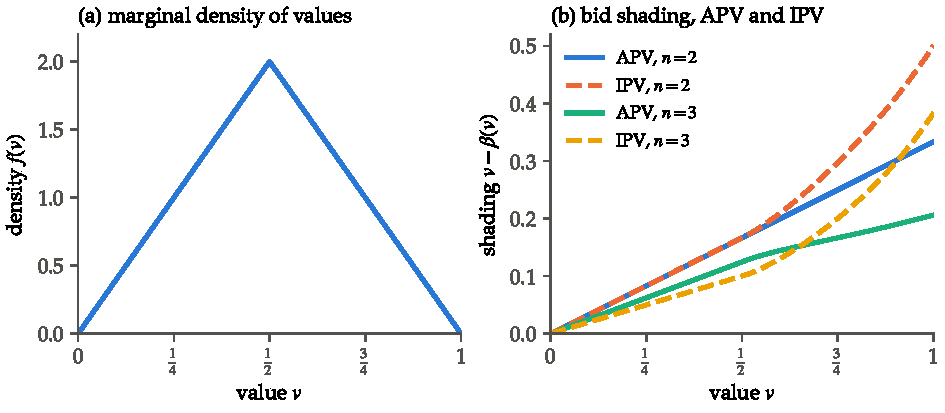
\includegraphics[width=\textwidth]{figures/ch15/lpv_design.pdf}
  \caption{The Monte Carlo design of \citet{LiPerrigneVuong2002}. Panel (a): the triangular marginal density
  of values when $V_i=Q+E_i$ with $Q\sim U[\frac14,\frac34]$ and $E_i\sim U[-\frac14,\frac14]$. Panel (b):
  bid shading $v-\beta(v)$ in the APV equilibrium (solid) and in the IPV equilibrium with the same marginal
  density (dashed), for $n=2$ and $n=3$. The APV bids use equations (10)--(12) of
  \citet{LiPerrigneVuong2002}, which we checked against a numerical solution of \eqref{eq:15-lpv-ode}.
  Our computation, with no random numbers (script \texttt{lpv\_design.py}).}\label{fig:15-lpv-design}
\end{figure}

Each replication draws 100 auctions with two bidders and 100 auctions with three bidders, which gives 500
bids. The experiment is replicated 1,000 times \citep[p.~179]{LiPerrigneVuong2002}. Each replication takes
less than three seconds \citep[p.~182]{LiPerrigneVuong2002}. The average first-step bandwidths $(h_G,h_g)$
are $(0.148,0.177)$ for $n=2$ and $(0.076,0.122)$ for $n=3$.

\casehead{Results} The median estimate of the inverse bid function tracks the truth closely and lies
slightly above it. The pointwise 90 percent band contains the true function except near the boundaries
(their Figures 1--2). The estimated marginal density follows the triangle except near the kink, where
kernel smoothing rounds the peak (their Figures 3--5). The winner's \emph{informational rent} in auction
$t$ is
\begin{equation}\label{eq:15-ir}
  \mathrm{IR}_t=\frac{v_{wt}-b_{wt}}{v_{wt}},
\end{equation}
with $v_{wt}$ and $b_{wt}$ the winner's value and bid \citep[eq.~(16)]{LiPerrigneVuong2002}. For $n=2$
the APV bid is $\frac23v$ on the whole support, so the true rent is exactly one third.
\Cref{tab:15-lpv-rents} reports the true mean rent and the distribution across replications of the
estimated average rent. The APV estimator slightly overstates the rent, consistent with the slight upward
bias in $\hat\xi$. Rents fall from $n=2$ to $n=3$, a competition effect.

\begin{table}[htbp]
\centering
\caption{Winners' informational rents in the Monte Carlo of \citet{LiPerrigneVuong2002}}\label{tab:15-lpv-rents}
\begin{tabular}{@{}lcccc@{}}
\toprule
 & \multicolumn{2}{c}{APV estimator (Table 1)} & \multicolumn{2}{c}{IPV estimator (Table 2)} \\
\cmidrule(lr){2-3}\cmidrule(lr){4-5}
 & $n=2$ & $n=3$ & $n=2$ & $n=3$ \\
\midrule
True mean IR & 33.33 & 23.47 & 33.33 & 23.47 \\
Estimated average IR & 36.76 & 26.96 & 38.65 & 29.11 \\
Empirical 5th percentile & 32.44 & 19.32 & 31.53 & 19.05 \\
Empirical 95th percentile & 41.18 & 34.69 & 49.33 & 44.97 \\
\bottomrule
\end{tabular}

\smallskip
\begin{minipage}{0.86\textwidth}
\footnotesize \textit{Notes.} Percent. The informational rent is \eqref{eq:15-ir}. Each column summarizes 1,000
replications, each with 100 two-bidder and 100 three-bidder auctions. The APV columns use the estimator
\eqref{eq:15-lpv-Ghat}--\eqref{eq:15-lpv-pseudo}. The IPV columns apply the estimator of
\citet{GuerrePerrigneVuong2000} to the same affiliated bids. Source: \citet[Tables~1 and~2]{LiPerrigneVuong2002}.
\end{minipage}
\end{table}

\casehead{Imposing independence on affiliated data} The authors then apply the IPV estimator of
\citet{GuerrePerrigneVuong2000} to the same simulated bids. The estimated inverse bid function matches the
truth for low bids but lies well above it for high bids (their Figures 6--7). The implied value density is
too dispersed (their Figures 8--9), and rents are overstated (\cref{tab:15-lpv-rents}). The authors report
overstatements of 17 and 24 percent for $n=2$ and $n=3$ \citep[p.~186]{LiPerrigneVuong2002}. Relative to
the true means in the table, the overstatements are 16 and 24 percent (our calculation).

A short calculation shows why. With $n=2$ the bid is $\frac23v$, so the marginal bid distribution is
$G(b)=F(\frac32b)$ with density $g(b)=\frac32f(\frac32b)$. The IPV inversion returns
\begin{equation*}
  \xi^{IPV}(b)=b+\frac{G(b)}{g(b)}=\frac23v+\frac23\,\frac{F(v)}{f(v)},\qquad v=\tfrac32b .
\end{equation*}
For $v\le\frac12$, $\frac{F(v)}{f(v)}=\frac{2v^2}{4v}=\frac v2$, so $\xi^{IPV}=v$ and low values are
recovered exactly. For $v>\frac12$, $\frac{F(v)}{f(v)}=\frac{1-2(1-v)^2}{4(1-v)}$. At $v=\frac34$ this is
$\frac78$, so $\xi^{IPV}=\frac12+\frac{7}{12}=\frac{13}{12}$ against a true value of $\frac34$. The
inversion explodes near the top because the marginal density vanishes there. The IPV model reads the
aggressive bidding of high types under affiliation as evidence of high values.

\casehead{Assessment} The paper extends the indirect approach to dependent values and supplies a usable
guide. Its limits are statistical and economic. The density of values is $n$-variate, so data demands grow
quickly with $n$, and estimation proceeds separately for each $n$. The estimator conditions on the number of
bidders, so it cannot by itself say how affiliation interacts with entry. Under APV, bids can fall as $n$
rises \citep{PinkseTan2005}. Regressions of bids on $n$ therefore cannot separate private from common values
(\cref{sec:15-cv-tests}). Finally, correlation in values may come from auction features that bidders observe
and the econometrician does not. That alternative is observationally equivalent to affiliation with a fixed
$n$, and \cref{sec:15-uh} treats it.

\subsection{What the two highest bids reveal}\label{sec:15-apv-top2}

Many first-price data sets record only the winning bid, or the two highest bids. Procurement agencies keep
the second-lowest bid in case the winner defaults. Participants also track the gap between the top two
bids, which they call ``money left on the table'' \citep[p.~2123]{AtheyHaile2002}. Two bids suffice for
part of the identification problem. \Cref{eq:15-lpv-foc} involves only the distribution of the
highest rival bid given one's own bid. In equilibrium the top two bids come from the bidders with the top
two values. Let $I^{(n:n)}$ denote the identity of the winner.

\begin{proposition}[{\citealp[Lemma~1, Theorem~7 and Corollary~1]{AtheyHaile2002}}]\label{prop:15-top2}
Consider the APV model of the first-price auction, and suppose the two highest bids are observed. If
bidders are asymmetric, suppose the identity of the winner is also observed.
\begin{enumerate}[label=(\roman*)]
  \item The equilibrium bid functions $\beta_i$, $i=1,\dots,n$, are identified.
  \item With symmetric bidders, the joint distribution of $(V^{(n:n)},V^{(n-1:n)})$ is identified.
  \item With symmetric bidders, the joint distribution $F$ of values is not identified if any lower bid is
  unobserved.
\end{enumerate}
\end{proposition}

\begin{proof}
(i) Take bidder 1 and a bid $b$ in the support of $B_1$. Multiply the numerator and denominator of the
markdown by the density of $B_1$ at $b$. Then translate each event into events about the top two bids:
\begin{align*}
  \frac{G_{M_1\mid B_1}(b\mid b)}{g_{M_1\mid B_1}(b\mid b)}
  &=\frac{\frac{\partial}{\partial y}\Pr\left(M_1\le b,\ B_1\le y\right)\big|_{y=b}}
  {\frac{\partial^2}{\partial x\,\partial y}\Pr\left(M_1\le x,\ B_1\le y\right)\big|_{x=y=b}}\\[2pt]
  &=\frac{\frac{\partial}{\partial x}\Pr\left(B^{(n:n)}\le x,\ I^{(n:n)}=1\right)\big|_{x=b}}
  {\frac{\partial^2}{\partial x\,\partial y}\Pr\left(B^{(n-1:n)}\le x,\ B^{(n:n)}\le y,\ I^{(n:n)}=1\right)\big|_{x=y=b}}.
\end{align*}
For the numerator, $\Pr(B^{(n:n)}\le x,\,I^{(n:n)}=1)=\Pr(B_1\le x,\,M_1<B_1)$, whose derivative at $x=b$
is $\Pr(M_1<b\mid B_1=b)\,g_{B_1}(b)$. For the denominator, take $x<y$. The event
$\{B^{(n-1:n)}\le x,\,B^{(n:n)}\le y,\,I^{(n:n)}=1\}$ equals $\{M_1\le x,\,B_1\le y\}$ minus
$\{M_1\le x,\,B_1\le M_1\}$. The probability of the second set does not depend on $y$. So the cross
partial equals the joint density of $(M_1,B_1)$ at $(x,y)$, and we let $x\uparrow y=b$. Both final
expressions involve only the top two bids and the winner's identity. The markdown is therefore identified,
and with it $\beta_1^{-1}(b)=b+\frac{G_{M_1\mid B_1}(b\mid b)}{g_{M_1\mid B_1}(b\mid b)}$ for almost every $b$.

(ii) With symmetric bidders the top two bids are $\beta(V^{(n:n)})$ and $\beta(V^{(n-1:n)})$. Apply the
identified $\beta^{-1}$ to both.

(iii) The construction of \cref{thm:15-ah4} applies. Shift probability mass between small neighborhoods of
two value vectors that differ only in the $j$-th order statistic, for some $j<n-1$, and symmetrize over
permutations. The new distribution is exchangeable. The distribution of the highest rival value, and hence
every bidder's best response, is unchanged. Only the unobserved order statistic $V^{(j:n)}$ changes its
distribution, so observables are unchanged \citep[proof of Theorem~3.4]{AtheyHaile2007}.
\end{proof}

Part (ii) is more useful than it looks. The joint law of the top two values determines the revenue from a
second-price or ascending auction and the effect of a reserve price. It also determines the outcome under
many other selling mechanisms \citep[p.~2124]{AtheyHaile2002}. Part (i) delivers the bid functions, which measure the wedge
between bids and values. Part (iii) is a limit. Bid functions depend only on the distribution of the
highest rival bid, so they carry no information about the distribution of lower bids. The design of an
optimal auction needs the full $F$ and therefore all bids. The two highest bids also suffice for a test of
private against common values, which \cref{thm:15-ah11} develops. \citet[Section~3.3.2]{AtheyHaile2007} note
that estimators built on part (i) had not yet been explored.

\subsection{Asymmetric affiliated private values: Campo, Perrigne and Vuong (2003)}\label{sec:15-apv-cpv}

\casehead{Question} Federal auctions of offshore oil leases allowed firms to bid jointly as consortia.
Joint bidding may pool capital and information, and it may create ex ante asymmetry among bidders.
\citet{CampoPerrigneVuong2003} ask whether an asymmetric APV model can be identified and estimated without
solving its equilibrium. They then use joint and solo bids to measure asymmetry, affiliation, unobserved
tract heterogeneity and informational rents. They also confront the pure common value model that dominated
earlier work on these auctions.

\casehead{Model} There are two types. Type 1 (strong, here joint bidders) has $n_1$ bidders and type 0
(weak, here solo bidders) has $n_0$ bidders, with $n_1+n_0=n\ge2$. Values
$(v_{11},\dots,v_{1n_1},v_{01},\dots,v_{0n_0})$ are drawn from an absolutely continuous distribution $F$ on
$[\underline v,\bar v]^n$. The distribution is affiliated and exchangeable within each type
\citep[Section~2.1]{CampoPerrigneVuong2003}. Let $\mathcal P$ denote this set of distributions. Within a
type, bidders use the same strictly increasing strategy, $s_1$ or $s_0$. Let $y_1^\ast$ be the highest value
among the other type-1 bidders and $y_0$ the highest type-0 value. A type-1 bidder with value $v_1$ solves
\begin{equation*}
  \max_b\ (v_1-b)\,\Pr\bigl(y_1^\ast\le s_1^{-1}(b),\ y_0\le s_0^{-1}(b)\mid v_1\bigr).
\end{equation*}
The first-order conditions form a system of two differential equations with boundary conditions
$s_1(\underline v)=s_0(\underline v)=\underline v$ and $s_1(\bar v)=s_0(\bar v)$, their equations (1)--(2).
The system is intractable in general. Under conditions that cover this model, an equilibrium in monotone pure
strategies nevertheless exists \citep{RenyZamir2004}. The inversion below assumes that bidders play such an
equilibrium and that each bid distribution is continuous and strictly increasing. Conditioning on a bidder's bid is
then the same as conditioning on her value. With independent values it reduces to the asymmetric IPV system of
\cref{prop:14-maskin-riley}, studied by \citet{MaskinRiley2000}, and with one type it reduces to
\eqref{eq:15-lpv-ode}.

\casehead{Inversion} Let $B_1^\ast$ be the highest bid among the other type-1 bidders and $B_0$ the highest
type-0 bid. Define $G_{B_1^\ast,B_0\mid b_1}(X,Y\mid x)=\Pr(B_1^\ast\le X,\,B_0\le Y\mid b_1=x)$. Since bids
are strictly increasing in values,
\begin{equation*}
  G_{B_1^\ast,B_0\mid b_1}(X,X\mid x)=F_{y_1^\ast,y_0\mid v_1}\bigl(s_1^{-1}(X),\,s_0^{-1}(X)\mid s_1^{-1}(x)\bigr).
\end{equation*}
The total derivative in the common threshold $X$ is
\begin{equation*}
  \frac{d}{dX}G_{B_1^\ast,B_0\mid b_1}(X,X\mid x)
  =\frac{\partial F_{y_1^\ast,y_0\mid v_1}}{\partial y_1^\ast}\frac{1}{s_1'\bigl(s_1^{-1}(X)\bigr)}
  +\frac{\partial F_{y_1^\ast,y_0\mid v_1}}{\partial y_0}\frac{1}{s_0'\bigl(s_0^{-1}(X)\bigr)}.
\end{equation*}
This is exactly the bracket in the type-1 first-order condition. Substituting gives
\begin{equation}\label{eq:15-cpv-foc}
  v_1=\xi_1(b_1;\bm G)\equiv b_1+\frac{G_{B_1^\ast,B_0\mid b_1}(b_1,b_1\mid b_1)}
  {\frac{d}{dX}G_{B_1^\ast,B_0\mid b_1}(X,X\mid b_1)\big|_{X=b_1}},
\end{equation}
their equation (4). The weak type's inverse $\xi_0(b_0;\bm G)$ is the same expression with
$(B_1,B_0^\ast)$ in place of $(B_1^\ast,B_0)$, their equation (5). Two features distinguish
\eqref{eq:15-cpv-foc} from \eqref{eq:15-lpv-foc}. The conditioning distribution is trivariate, since it
involves the bidder's own bid and the highest bid of each type. The denominator is a total derivative and not
a density.

\begin{proposition}[{\citealp[Proposition~1]{CampoPerrigneVuong2003}}]\label{prop:15-cpv}
The asymmetric APV model is identified. Let $\bm G$ have support $[\underline b,\bar b]^n$. It can be
rationalized by an asymmetric APV model with $F\in\mathcal P$ if and only if two conditions hold.
\begin{enumerate}[label=(\roman*)]
  \item $\bm G\in\mathcal P$.
  \item $\xi_1(\cdot;\bm G)$ and $\xi_0(\cdot;\bm G)$ are strictly increasing on $[\underline b,\bar b]$, with
  $\xi_1(\bar b;\bm G)=\xi_0(\bar b;\bm G)$.
\end{enumerate}
The rationalizing distribution is
$F(\bm v_1,\bm v_0)=\bm G\bigl(\xi_1^{-1}(\bm v_1;\bm G),\xi_0^{-1}(\bm v_0;\bm G)\bigr)$.
\end{proposition}

The proof follows that of \cref{prop:15-lpv}. The common upper endpoint in (ii) reflects the boundary
condition $s_1(\bar v)=s_0(\bar v)$. Identification is nonparametric and requires neither solving nor
approximating the equilibrium. Because $\mathcal P$ contains the distributions that are exchangeable across all
$n$ bidders, the symmetric model is nested and can be tested against the asymmetric one.

\casehead{Estimator} The conditioning on $b_1$ drops out of the ratio in \eqref{eq:15-cpv-foc}, which equals
\begin{equation}\label{eq:15-cpv-ratio}
  \frac{\Pr(B_1^\ast\le b_1,\ B_0\le b_1,\ b_1=b_1)}
  {\Pr(B_1^\ast=b_1,\ B_0\le b_1,\ b_1=b_1)+\Pr(B_1^\ast\le b_1,\ B_0=b_1,\ b_1=b_1)},
\end{equation}
where each ``$=$'' denotes a density \citep[eq.~(6)]{CampoPerrigneVuong2003}. With $T$ auctions of a given
configuration $(n_1,n_0)$, the numerator is estimated by
\begin{equation*}
  \hat G_1(x,y,z)=\frac{1}{h_{G1}T}\sum_{t=1}^{T}\frac{1}{n_1}\sum_{i=1}^{n_1}
  \indic(B_{1it}^\ast\le x)\,\indic(B_{0t}\le y)\,\mathcal K\left(\frac{z-B_{1it}}{h_{G1}}\right).
\end{equation*}
The two terms of the denominator replace one indicator at a time by a kernel:
\begin{align*}
  \hat D_{11}(x,y,z)&=\frac{1}{h_{g1}^2T}\sum_{t=1}^{T}\frac{1}{n_1}\sum_{i=1}^{n_1}
  \mathcal K\left(\frac{x-B_{1it}^\ast}{h_{g1}}\right)\indic(B_{0t}\le y)\,\mathcal K\left(\frac{z-B_{1it}}{h_{g1}}\right),\\
  \hat D_{12}(x,y,z)&=\frac{1}{h_{g1}^2T}\sum_{t=1}^{T}\frac{1}{n_1}\sum_{i=1}^{n_1}
  \indic(B_{1it}^\ast\le x)\,\mathcal K\left(\frac{y-B_{0t}}{h_{g1}}\right)\mathcal K\left(\frac{z-B_{1it}}{h_{g1}}\right).
\end{align*}
The pseudo-value of a type-1 bid is
$\hat V_{1it}=B_{1it}+\frac{\hat G_1(B_{1it},B_{1it},B_{1it})}{\hat D_{11}(B_{1it},B_{1it},B_{1it})+\hat
D_{12}(B_{1it},B_{1it},B_{1it})}$, their equation (7), and type 0 is symmetric. The second step estimates
bivariate densities of pairs of values within and across types \citep[eqs.~(9)--(11)]{CampoPerrigneVuong2003}.
Because bid data are skewed, the authors work with $d=\ln(1+b)$. If $D=\ln(1+B)$, densities in $b$ equal
densities in $d$ divided by $1+b$. Then the markdown in $b$ is $(1+b)$ times the markdown in $d$, and
\begin{equation*}
  v=b+(1+b)\frac{G_D}{g_D}=e^{d}\left(1+\frac{G_D}{g_D}\right)-1,
\end{equation*}
which is their equation (12). They use triweight kernels, rule-of-thumb bandwidths of the form
$c\,(n_1T)^{-\frac15}$ and $c\,(n_1T)^{-\frac16}$ with $c=2.978\times1.06\,\hat\sigma$, and trimming within one
bandwidth of the boundaries \citep[pp.~188--189]{CampoPerrigneVuong2003}.

\casehead{Unobserved tract heterogeneity} Tracts differ in observed characteristics $Z$ and unobserved
characteristics $W$. Without restrictions, variation in $W$ cannot be separated from variation in private
values. \citet[Section~3.2]{CampoPerrigneVuong2003} impose the following.

\begin{assumption}[{\citealp[Section~3.2]{CampoPerrigneVuong2003}}]\label{ass:15-cpv-uh}
(i) The numbers of bidders of each type are deterministic functions of tract characteristics,
$n_1=n_1(Z,W)$ and $n_0=n_0(Z,W)$. (ii) Conditional on $(Z,n_1,n_0)$, values do not depend on $W$:
$F(\cdot\mid Z,W)=F(\cdot\mid Z,n_1,n_0)$.
\end{assumption}

Part (i) holds in entry models in which firms decide to participate before learning their values. Part (ii)
says that the bidder configuration is a sufficient statistic for the unobserved tract characteristics.
Estimation conditional on $(n_1,n_0)$ is then valid. The same idea, using an endogenous count as a control
for unobservables, underlies the instrumental approach of \citet{HaileHongShum2003} in
\cref{sec:15-cv-tests}. It also has a cost. Under \cref{ass:15-cpv-uh} the value distribution of joint bidders
may differ between $(2,0)$ and $(1,1)$ auctions because the tracts differ. A comparison of the marginal
densities of a type across configurations therefore tests for unobserved heterogeneity. A comparison of joint
and solo densities within the $(1,1)$ configuration tests for asymmetry.

\casehead{The asymmetric pure common value model} Pure common values had been the standard model for
offshore leases. \citet{CampoPerrigneVuong2003} derive a sharp restriction for two bidders. The tract has
common value $V$. Bidder $i\in\{0,1\}$ receives a signal $\sigma_i$, and the signals are independent given
$V$ but not identically distributed. Let $V(\sigma_1,\sigma_0)=\E[V\mid\sigma_1,\sigma_0]$. Bidder 1 wins
when $\sigma_0\le s_0^{-1}(b_1)$, so her first-order condition is
\begin{equation*}
  -F_{\sigma_0\mid\sigma_1}\bigl(s_0^{-1}(b_1)\mid\sigma_1\bigr)
  +\bigl[V\bigl(\sigma_1,s_0^{-1}(b_1)\bigr)-b_1\bigr]
  \frac{f_{\sigma_0\mid\sigma_1}\bigl(s_0^{-1}(b_1)\mid\sigma_1\bigr)}{s_0'\bigl(s_0^{-1}(b_1)\bigr)}=0,
\end{equation*}
their equation (14). The argument leading to \eqref{eq:15-lpv-foc} turns it into
\begin{equation}\label{eq:15-cpv-cv}
  V\bigl(\sigma_1,s_0^{-1}(b_1)\bigr)=b_1+\frac{G_{b_0\mid b_1}(b_1\mid b_1)}{g_{b_0\mid b_1}(b_1\mid b_1)}=\xi_1(b_1;\bm G),
  \qquad
  V\bigl(s_1^{-1}(b_0),\sigma_0\bigr)=\xi_0(b_0;\bm G),
\end{equation}
their equations (16)--(17). The right sides are the same as in the APV model with two bidders. Only the
interpretation of the left sides changes. A bivariate distribution of $(b_1,b_0)$ is
\emph{quasi-symmetric} if $\Pr(b_1\le b_0\mid b_1\le b,\,b_0\le b)=\Pr(b_1\ge b_0\mid b_1\le b,\,b_0\le
b)$ for every $b$. Exchangeable distributions are quasi-symmetric, but not conversely.

\begin{proposition}[{\citealp[Proposition~2]{CampoPerrigneVuong2003}}]\label{prop:15-cpv-quasisym}
If observed bids are equilibrium bids of an asymmetric pure common value model with two bidders, their joint
distribution is quasi-symmetric. Quasi-symmetry is equivalent to $\xi_1(b;\bm G)=\xi_0(b;\bm G)$ for every
$b$. The asymmetric pure common value model is observationally equivalent to an asymmetric APV model with a
quasi-symmetric value distribution and identical equilibrium strategies.
\end{proposition}

\begin{proof}
At a common bid $b$, bidder 1's signal is $s_1^{-1}(b)$ and bidder 0's is $s_0^{-1}(b)$. Both left sides of
\eqref{eq:15-cpv-cv} then equal $V\bigl(s_1^{-1}(b),s_0^{-1}(b)\bigr)$, so $\xi_1(b)=\xi_0(b)$. To link this to
quasi-symmetry, let $G(x,y)=\Pr(b_1\le x,\,b_0\le y)$ with density $g$, and let $\partial_1G$ and $\partial_2G$
be its partial derivatives. Then
$G_{b_0\mid b_1}(y\mid x)=\frac{\partial_1G(x,y)}{g_{b_1}(x)}$ and $g_{b_0\mid b_1}(y\mid x)=\frac{g(x,y)}{g_{b_1}(x)}$,
so
\begin{equation*}
  \xi_1(b)-b=\frac{\partial_1G(b,b)}{g(b,b)},\qquad \xi_0(b)-b=\frac{\partial_2G(b,b)}{g(b,b)} .
\end{equation*}
Hence $\xi_1=\xi_0$ if and only if $\partial_1G(b,b)=\partial_2G(b,b)$ for all $b$. Next,
\begin{align*}
  \Pr(b_1\le b_0\le b)&=\int^{b}\!\!\int^{y}g(x,y)\,dx\,dy=\int^{b}\partial_2G(y,y)\,dy,\\
  \Pr(b_0\le b_1\le b)&=\int^{b}\partial_1G(x,x)\,dx .
\end{align*}
These two probabilities are equal for every $b$ if and only if $\partial_1G(b,b)=\partial_2G(b,b)$ for every
$b$. Ties have probability zero, so equal probabilities mean each is half of $G(b,b)$, which is
quasi-symmetry. For the last claim, define private values $\tilde v_i=\xi_i(b_i)$. They form a
quasi-symmetric distribution, and the common strategy $\xi^{-1}$ satisfies both APV first-order conditions.
\end{proof}

Setting $b=\bar b$ gives $\Pr(b_1\le b_0)=\frac12$. Each bidder wins half of the time, however different
their information. The same property holds in the extreme case with one perfectly informed bidder, where the
uninformed bidder's mixed strategy replicates the informed bid distribution (\cref{prop:14-emw}). The
proposition yields a simple test of the pure common value model with two bidders, whatever the asymmetry.

\casehead{Setting and data} The federal government has auctioned oil and gas rights on the Outer Continental
Shelf (OCS) since 1954. \citet{CampoPerrigneVuong2003} study wildcat sales in the Gulf of Mexico off Louisiana. Areas
are divided into tracts, usually of 5,000 or 5,760 acres, sold simultaneously by first-price sealed bid. The
reserve price of \$15 per acre is not regarded as screening participation (their footnote 10). Joint bidding
affected fewer than 20 percent of auctions before 1970 and more than 80 percent after. A typical joint bid
involves two or three firms. From December 1975, the eight largest firms were barred from bidding jointly
with each other (their footnote 11). The sample covers auctions from December 1972 to 1979. It excludes later
years because the rules changed, and two early sales with unusual water depth (their footnote 12). The
authors keep auctions with exactly two bidders. This gives 227 auctions: 60 with two joint bids, 55 with two
solo bids and 112 with one of each. Bids are in 1972 dollars per acre. \Cref{tab:15-cpv-stats} reproduces
their Table I.

\begin{table}[htbp]
\centering
\caption{Bids in two-bidder OCS wildcat auctions, 1972--1979 (dollars per acre)}\label{tab:15-cpv-stats}
\begin{tabular}{@{}lrrrrrr@{}}
\toprule
 & Obs. & Mean & Std.\ dev. & Minimum & Maximum & Within s.d. \\
\midrule
All bids & 454 & 687.30 & 1,431.31 & 19.51 & 20,751.32 & 1,258.91 \\
Joint bids & 232 & 837.32 & 1,717.54 & 21.46 & 20,751.32 & \\
Solo bids & 222 & 532.53 & 1,033.20 & 19.51 & 11,019.08 & \\
Joint vs.\ joint & 120 & 875.13 & 2,056.12 & 33.94 & 20,751.32 & 2,011.99 \\
Joint vs.\ solo & 112 & 796.83 & 1,266.32 & 21.46 & 6,377.94 & \\
Solo vs.\ joint & 112 & 603.28 & 1,226.61 & 19.51 & 11,019.08 & \\
Solo vs.\ solo & 110 & 456.45 & 788.19 & 20.80 & 7,009.10 & 747.43 \\
\bottomrule
\end{tabular}

\smallskip
\begin{minipage}{0.92\textwidth}
\footnotesize \textit{Notes.} Bids in 1972 dollars per acre. ``Joint vs.\ solo'' means joint bids in auctions whose
other bidder is solo. The within standard deviation is computed within auctions. Source:
\citet[Table~I]{CampoPerrigneVuong2003}.
\end{minipage}
\end{table}

Joint bids are higher on average than solo bids. Each type bids more when facing a joint bidder. A test of
equal means of joint and solo bids in the 112 mixed auctions gives $t=1.66$, a weak rejection at the 10
percent level \citep[p.~190]{CampoPerrigneVuong2003}. Joint bidders won 63 of the 112 mixed auctions. This
share exceeds one half at the 10 percent level in a one-sided test. The within-auction standard deviation is
70 to 98 percent of the total, and 98 percent in auctions with two joint bidders. So much of the variation
across tracts is explained by the bidder configuration. In log-bid regressions, the three bidding-structure
dummies are jointly significant. Equality of the 16 sale dummies is nearly accepted, and neither the 1973
oil shock nor the 1975 ban has a significant effect \citep[p.~191]{CampoPerrigneVuong2003}.

\casehead{Testing pure common values} By \cref{prop:15-cpv-quasisym}, the joint bidder should win half of
the mixed auctions. The authors split the 112 mixed auctions in half. In the 56 auctions with both bids below
\$460 per acre, the joint bidder wins 28 times. In the 56 auctions with at least one bid above \$460, it wins
35 times. Quasi-symmetry requires a winning probability of one half in each subset. In the second subset,
$t=1.87$ rejects \citep[p.~195]{CampoPerrigneVuong2003}. As a check, the share $\frac{35}{56}=0.625$ has
standard error $\sqrt{\frac{0.25}{56}}=0.067$ under the null, which reproduces $t=1.87$. The pure common
value model is rejected for these auctions. A general model with values $U(\sigma_i,V)$ is not rejected, since
it is not identified \citep{LaffontVuong1996}.

\casehead{Results with one type} The $(2,0)$ and $(0,2)$ configurations are symmetric APV models, estimated as
in \cref{sec:15-apv-lpv}. Three and six auctions are trimmed. Both estimated inverse bid functions are
increasing, so the APV model is not rejected. The function for joint bidders facing joint bidders lies to the
right of that for solo bidders facing solo bidders. For the same value, a joint bidder facing a joint bidder
bids more. The value distribution of joint bidders first-order stochastically dominates that of solo bidders
in a one-sided Kolmogorov-Smirnov test. The trimmed pseudo-values have mean \$2,195.14 for joint bidders and
\$1,027.90 for solo bidders (their footnote 19). The test of \citet{BlumKieferRosenblatt1961} rejects
independence of the two values in every case. The statistic is 6.57 on bids and 4.69 on trimmed pseudo-values
for joint pairs. For solo pairs it is 9.52 and 6.92 \citep[p.~197]{CampoPerrigneVuong2003}.

\casehead{Results with both types} In the $(1,1)$ case the starred maxima are void, and the inversions reduce
to $\xi_{10}(b_1)=b_1+\frac{G_{b_0\mid b_1}(b_1\mid b_1)}{g_{b_0\mid b_1}(b_1\mid b_1)}$ and its mirror image
\citep[eqs.~(18)--(19)]{CampoPerrigneVuong2003}. After trimming 21 auctions, 91 remain. Both estimated
inverse functions increase. The solo bidder's function lies to the right of the joint bidder's, especially
above \$500 per acre. For the same value, a solo bidder bids more aggressively. This again contradicts
quasi-symmetry. The value densities of the two types are close (\cref{fig:15-cpv-xi}, panel b). Trimmed
pseudo-values average \$1,208.73 for joint and \$1,161.62 for solo bidders (their footnote 21). A
Kolmogorov-Smirnov test does not reject equal distributions (their footnote 22). Asymmetry in values is weak.
The weak bidder's lighter shading, that is, its more aggressive bidding, is the response that
\cref{prop:14-maskin-riley} predicts \citep[p.~199]{CampoPerrigneVuong2003}. It does
not produce inefficient allocations in the sample. Each type also adapts to its rival. A joint bidder bids
more aggressively against a joint bidder, and a solo bidder bids slightly more aggressively against a joint
bidder.

\begin{figure}[htbp]
  \centering
  \begin{subfigure}[b]{0.48\textwidth}
    \centering
    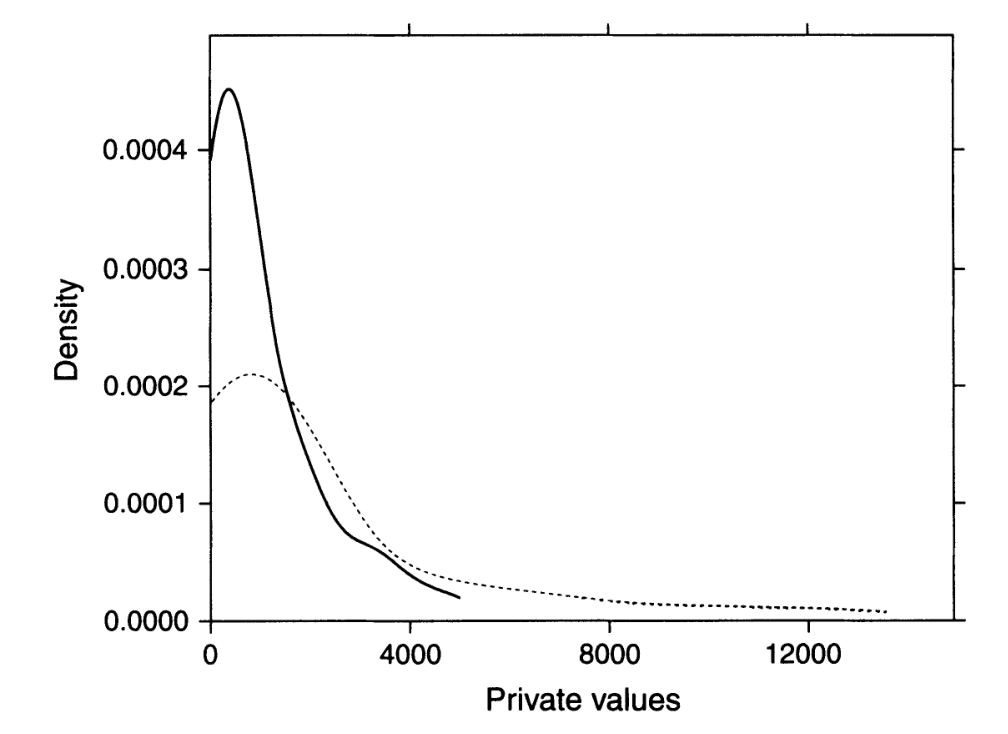
\includegraphics[width=\textwidth]{figures/ch15/cpv_fig2.png}
    \caption{Symmetric configurations: joint vs.\ joint (dashed), solo vs.\ solo (solid)}
  \end{subfigure}\hfill
  \begin{subfigure}[b]{0.48\textwidth}
    \centering
    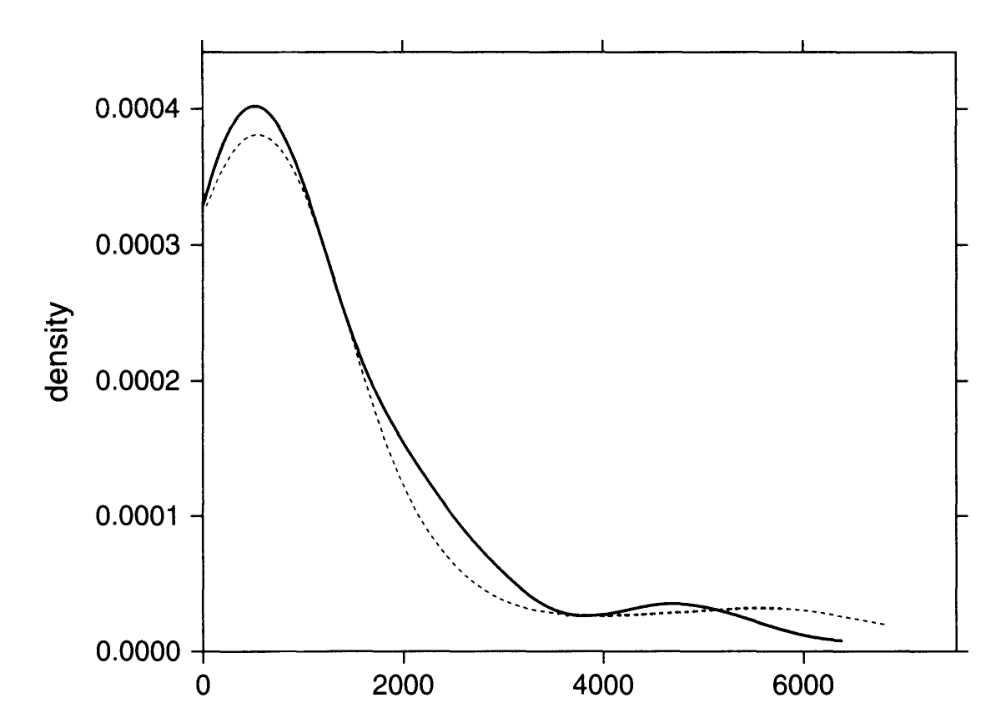
\includegraphics[width=\textwidth]{figures/ch15/cpv_fig4.png}
    \caption{Mixed configuration: joint (dashed), solo (solid)}
  \end{subfigure}
  \caption{Estimated marginal densities of private values in OCS wildcat auctions, dollars per acre. The
  horizontal axes differ across panels. In symmetric auctions the joint bidders' values are far more dispersed
  than the solo bidders'. In mixed auctions the two densities are close. The contrast between panels points to
  unobserved tract heterogeneity across configurations. Source: \citet{CampoPerrigneVuong2003}, Figures 2
  and 4.}\label{fig:15-cpv-xi}
\end{figure}

\casehead{Unobserved heterogeneity and rents} Under \cref{ass:15-cpv-uh}, comparing a type's value density
across configurations detects unobserved tract heterogeneity. Kolmogorov-Smirnov statistics are 0.1917 for
joint bidders in $(2,0)$ against $(1,1)$ auctions and 0.0965 for solo bidders in $(0,2)$ against $(1,1)$
auctions \citep[p.~200]{CampoPerrigneVuong2003}. The authors read the first as a clear rejection. Tracts
that attract two joint bidders are more valuable than tracts that attract one bidder of each type. The
differences in \cref{tab:15-cpv-stats} thus reflect both asymmetry and tract heterogeneity, with
heterogeneity the larger force. Winners' informational rents \eqref{eq:15-ir} average 65.07 percent across 197
winners (their Table II). They are 65.50 percent for joint and 64.59 percent for solo winners. So the
government captures about 35 percent of the winner's willingness to pay. In dollars, joint winners earn
\$1,954.42 per acre and solo winners \$1,151.40, because joint winners have higher values
\citep[p.~201]{CampoPerrigneVuong2003}.

\casehead{Interpretation and critiques} Asymmetry between joint and solo bidders is weak. A ban on joint bidding
would therefore change little if participation stayed the same. The authors argue that joint bidding raised
revenue by increasing participation. The paper's contribution is methodological. It shows that the indirect
approach handles asymmetric bidders whose equilibrium cannot be computed, and it gives a usable test of pure
common values. The limits are severe in practice. The trivariate objects in \eqref{eq:15-cpv-foc} force the
analysis to two-bidder auctions. With three bidders only 18 to 60 auctions would be available per
configuration (their footnote 16). Types are binary and the configuration is taken as exogenous to values
given the tract. The private value assumption for oil leases is contested. \citet{HendricksPinksePorter2003}
find bidding on earlier OCS auctions more consistent with common values (\cref{sec:15-cv-hp}).

\subsection{Asymmetric independent private values with all bids}\label{sec:15-apv-asym}

Independence simplifies the inversion and lowers data requirements. Let bidder $j$'s bid have distribution
$G_j$ and density $g_j$. With independent values, bids are independent, so
$G_{M_i\mid B_i}(m\mid b)=\prod_{j\ne i}G_j(m)$. Differentiating the product,
\begin{align*}
  g_{M_i\mid B_i}(m\mid b)&=\sum_{k\ne i}g_k(m)\prod_{j\ne i,k}G_j(m),\\
  \frac{G_{M_i\mid B_i}(b\mid b)}{g_{M_i\mid B_i}(b\mid b)}
  &=\frac{\prod_{j\ne i}G_j(b)}{\sum_{k\ne i}g_k(b)\prod_{j\ne i,k}G_j(b)}
  =\left[\sum_{j\ne i}\frac{g_j(b)}{G_j(b)}\right]^{-1}.
\end{align*}
The inverse bid function is therefore
\begin{equation}\label{eq:15-asym-xi}
  v_i=\xi_i(b_i)=b_i+\left[\sum_{j\ne i}\frac{g_j(b_i)}{G_j(b_i)}\right]^{-1},
\end{equation}
the inverse form of \eqref{eq:14-asym-foc}. Each value depends on its own bid and on the univariate
distributions of rivals' bids. When all bids and bidder identities are observed, each $F_i$ is identified
by $F_i(v)=G_i(\xi_i^{-1}(v))$ \citep[Theorem~3.1(ii)]{AtheyHaile2007}.

Estimation must condition on the set of opponents, because a change in their identities changes the
strategy being inverted. With fully bidder-specific distributions, each set of bidders is treated separately.
This requires many auctions with the same bidder set. A practical compromise groups bidders into a few
types, with exchangeability within a type, as with joint and solo bidders or loggers and mills
\citep[Section~3.2.2]{AtheyHaile2007}. All auctions with the same number of bidders of each type can then be
pooled. Asymmetry can also come from bidder covariates, such as the distance from a contractor's plant to the
project. With discrete covariates this is the approach by types again. With continuous covariates the bid
distributions are estimated conditional on them by kernel or sieve methods. The timber study of
\cref{sec:15-als} applies \eqref{eq:15-asym-xi} with parametric bid distributions.

\citet{FlambardPerrigne2006} apply the procurement version nonparametrically to snow removal contracts in
Montreal \citep[p.~102]{HortacsuPerrigne2021}. In a low-bid auction bidder $i$ wins when every rival bids
more, and the same steps give
\begin{equation*}
  c_i=b_i-\left[\sum_{j\ne i}\frac{g_j(b_i)}{1-G_j(b_i)}\right]^{-1}.
\end{equation*}
Firms are classified by their location relative to the job, and participation, winning probabilities and bid
distributions differ across the classes. The estimated cost difference between the classes is about 6.5
percent. It leads to an inefficient allocation in 24 percent of the auctions. A subsidy to the weak,
high-cost firms that restores symmetry would raise the share of contracts they win by 61 percent. With a cost
of public funds taken into account, the overall procurement cost would fall by 1.34 percent under exogenous
participation.

Equilibrium imposes testable restrictions. With independence and a common support of values,
\cref{thm:15-ah-rational} requires bids to be independent, each $\xi_i$ to be increasing, and all $\xi_i$ to
share the same upper endpoint. The last restriction comes from the common support. It can fail in a valid
equilibrium if supports differ. \citet[Section~5.1]{AtheyHaile2007} give an example, which we verify. Let
$n=2$ with bid distributions $G_1(b)=b$ and $G_2(b)=b^2$ on $[0,1]$. Then \eqref{eq:15-asym-xi} gives
\begin{equation*}
  \xi_1(b)=b+\frac{G_2(b)}{g_2(b)}=b+\frac b2=\frac32b,
  \qquad
  \xi_2(b)=b+\frac{G_1(b)}{g_1(b)}=2b .
\end{equation*}
The implied value distributions are $F_1(v)=G_1(\frac23v)=\frac23v$ on $[0,\frac32]$ and
$F_2(v)=G_2(\frac v2)=\frac{v^2}{4}$ on $[0,2]$. Each strategy is a best response. Bidder 1 maximizes
$(v-b)b^2$, so $v=\frac32b$, and bidder 2 maximizes $(v-b)b$, so $v=2b$. Yet $\xi_1(1)=\frac32\ne2=\xi_2(1)$.
Equivalently, the densities of the highest rival bid differ at the top, $g_{M_1}(1)=g_2(1)=2$ and
$g_{M_2}(1)=g_1(1)=1$, so the boundary condition \eqref{eq:15-boundary-test} fails.
Allowing supports to differ across bidders restores identification in such cases. If the lower ends of the
supports also differ, some bidders may never win, and little can be learned about them
\citep[Section~5.1]{AtheyHaile2007}.

\section{Common Values: Limits of Identification and Tests}\label{sec:15-cv}

With common values, information about each bidder's value is dispersed among the bidders. Learning a
rival's signal would change a bidder's estimate of her own value (\cref{def:14-private-values}). Winning then
carries bad news, the winner's curse of \cref{sec:14-winners-curse}. Many policy questions turn on the joint
distribution of signals and values. Examples are the optimal reserve price, the revenue ranking of formats,
and whether restricting entry raises revenue. This section first shows how little bids reveal about that
distribution. It then shows that exogenous variation in competition still allows private values to be tested
against common values. Next it presents a positive identification result for procurement with interdependent
costs \citep{Somaini2020}. It ends with the evidence of \citet{HendricksPorter1988} on an auction with an
informed bidder.

\subsection{What bids can and cannot reveal}\label{sec:15-cv-limits}

Let bidder $i$ observe a signal $S_i$ about her value $V_i$. The primitive is the joint distribution
$F_{\bm S,\bm V}$ of signals and values. In the pure common value model $V_i=V_0$ for all $i$. We focus on
symmetric models. Let $Y_i=\max_{j\ne i}S_j$ and define the \emph{pivotal expected value}
\begin{equation*}
  v(s,y;n)=\E\left[V_i\mid S_i=s,\ Y_i=y;\ n\right],
\end{equation*}
the expected value of a bidder whose signal is $s$ and whose strongest rival has signal $y$. The dimension
count is discouraging. The primitive governs $2n$ random variables, or $n+1$ with pure common values, yet an
auction reveals at most $n$ bids \citep[Section~7.1]{AtheyHaile2007}.

Signals have only ordinal meaning. Any strictly increasing relabeling of a signal leaves behavior unchanged.
\citet[eq.~(8)]{AtheyHaile2002} use this freedom to impose the normalization
\begin{equation}\label{eq:15-cv-norm}
  v(s,s;n)=\E\left[V_i\mid S_i=\max_{j\ne i}S_j=s;\ n\right]=s .
\end{equation}
In the second-price auction the equilibrium bid is $v(s,s;n)$ (\cref{prop:14-mw-spa}). Under
\eqref{eq:15-cv-norm} it becomes $b(s)=s$, so bids reveal signals. In the first-price auction, the
first-order condition of \eqref{eq:14-apv-foc} holds with the pivotal expected value on the left:
\begin{equation}\label{eq:15-cv-foc}
  v(s_i,s_i;n)=b_i+\frac{G_{M\mid B}(b_i\mid b_i)}{g_{M\mid B}(b_i\mid b_i)}
\end{equation}
\citep[eq.~(7.2)]{AtheyHaile2007}. The right side is the same functional of bids as in the APV model. All
bids therefore identify the joint distribution of the random variables $v(S_i,S_i;n)$, $i=1,\dots,n$, and
nothing more.

\begin{proposition}[{\citealp{LaffontVuong1996}}]\label{prop:15-lv}
Fix $n$ and suppose the reserve price does not bind. Every symmetric affiliated value model of the
first-price auction with a strictly increasing equilibrium is observationally equivalent to a symmetric APV
model. Its private values are $\tilde V_i=v(S_i,S_i;n)$.
\end{proposition}

\begin{proof}
Bids are strictly increasing transformations of affiliated, exchangeable signals, so $\bm G$ is symmetric and
affiliated. By \eqref{eq:15-cv-foc}, $\xi(b;\bm G)=v\bigl(\beta^{-1}(b),\beta^{-1}(b);n\bigr)$, which is
strictly increasing in $b$. At $b=\beta(s)$ the ratio in \eqref{eq:15-cv-foc} equals $v(s,s;n)-\beta(s)$, which vanishes at
$\underline s$ because $\beta(\underline s)=v(\underline s,\underline s;n)$ by \eqref{eq:14-mw-fpa-bid2}. Both
conditions and the boundary condition of \cref{prop:15-lpv} hold, so an APV structure rationalizes
$\bm G$. Its values are $\xi(B_i;\bm G)=v(S_i,S_i;n)$.
\end{proof}

Conclusions drawn from bids with a fixed set of bidders and no reserve price therefore rest on a maintained
assumption of private or common values. Different maintained assumptions can justify a wide range of reserve
prices as optimal \citep[Section~7.1]{AtheyHaile2007}. Second-price and ascending auctions do no better.

\begin{proposition}[{\citealp[Corollary~2]{AtheyHaile2002}}]\label{prop:15-cv-nonid}
Consider the symmetric common value model of the second-price sealed-bid auction.
\begin{enumerate}[label=(\roman*)]
  \item The distribution of signals $F_{\bm S}$ is not identified from bids unless all bids are observed.
  \item The joint distribution $F_{\bm S,\bm V}$ is not identified from bids.
\end{enumerate}
\end{proposition}

\begin{proof}
Under \eqref{eq:15-cv-norm} bids equal signals. Part (i) is then \cref{thm:15-ah4} applied to the exchangeable
vector $\bm S$. For (ii), take two joint distributions with the same $F_{\bm S}$ and different conditional
laws of $\bm V$ given $\bm S$, both satisfying \eqref{eq:15-cv-norm}. In both, $b(s)=s$, so the
distributions of bids coincide.
\end{proof}

Ascending auctions are harder still. A normalization like \eqref{eq:15-cv-norm} can hold only in the initial
phase, before anyone exits. After each exit, bidders revise their planned exit prices in ways that depend on
$F_{\bm S,\bm V}$. With $n>2$ there is also a continuum of symmetric equilibria in undominated strategies
\citep{BikhchandaniHaileRiley2002}. Even the most restrictive common value model fails.

\begin{proposition}[{\citealp[Theorem~8]{AtheyHaile2002}}]\label{prop:15-ah8}
In an ascending auction, assume pure common values, independent and identically distributed signals, and the
equilibrium of \citet{MilgromWeber1982}. With $n$ fixed, the model is not identified from the observed bids,
even up to a normalization of signals.
\end{proposition}

\begin{proof}
Take $n=3$ and signals uniform on $[0,1]$. Let $s^{(1:3)}\le s^{(2:3)}\le s^{(3:3)}$ be the ordered signals.
Model A has $V_0=\frac{s_1+s_2+s_3}{3}$. Model B has
$\hat V_0=\frac{s^{(1:3)}}{3}+\frac{s^{(2:3)}}{6}+\frac{s^{(3:3)}}{2}$. In the Milgrom-Weber equilibrium each
bidder initially plans to exit at the expected value given that all signals equal her own. In both models
\begin{equation*}
  \E[V_0\mid S_1=S_2=S_3=s]=s=\frac s3+\frac s6+\frac s2,
\end{equation*}
so the first exit occurs at $B^{(1:3)}=s^{(1:3)}$ in both. Its distribution is $1-(1-b)^3$. The first exit
reveals $s^{(1:3)}$. Each remaining bidder then plans to exit at the expected value given her own signal $y$, the
revealed signal $s$, and a remaining rival with signal $y$. In Model A this is $\frac{s+2y}{3}$. In Model B it
is $\frac s3+\frac y6+\frac y2=\frac{s+2y}{3}$. The second exit therefore has the same conditional distribution
given $B^{(1:3)}$ in both models. The winner never exits, so the joint distribution of observed bids is the
same in both models.
\end{proof}

The two models differ in economically relevant ways. The optimal reserve price differs between them
\citep[footnote~38]{AtheyHaile2002}. In Model B a bidder's value depends less on her rivals' signals when her
own signal is the highest. This lowers the participation threshold for any reserve price and changes the
seller's objective \citep[Section~7.1]{AtheyHaile2007}.

\casehead{Identification with more structure} One route adds structure. In the symmetric \emph{mineral rights
model}, signals are independent given the common value. \citet{LiPerrigneVuong2000} add separability. For each
$n$ there are known constants $C$ and $D>0$ such that, under \eqref{eq:15-cv-norm}, $S_i=C+D(V_0+A_i)$, with
$(V_0,A_1,\dots,A_n)$ mutually independent and the $A_i$ identically distributed
\citep[p.~2126]{AtheyHaile2002}. Then \eqref{eq:15-cv-foc} reads
\begin{equation*}
  C+D\,(v_0+a_i)=b_i+\frac{G_{M\mid B}(b_i\mid b_i)}{g_{M\mid B}(b_i\mid b_i)} .
\end{equation*}
All bids identify the joint distribution of $(V_0+A_1,\dots,V_0+A_n)$. When the characteristic functions do
not vanish, the deconvolution argument of \cref{lem:15-kotlarski} separates the distributions of $V_0$ and
$A_i$. The argument fails when some bids are missing. Bids then reveal order statistics $V_0+A^{(i:n)}$,
which are dependent even though the $A_i$ are independent.

\citet{LiPerrigneVuong2000} apply this structure to wildcat leases of the Outer Continental Shelf
\citep[p.~129]{HortacsuPerrigne2021}. They estimate two versions. In the conditionally independent
private values version, each bidder's value is its signal $S_i=V_0A_i$, with $V_0$ independent of the
$A_i$, so logs are additive as above. In the pure common value version, the pivotal expected value is
log-linear in the log signal, and the model is identified only up to location and scale. In the first
version the recovered values are multiple indicators of $V_0$, a measurement-error problem that
deconvolution solves. The estimates show little affiliation. The variance of $\ln V_0$ is only 9.2
percent of the variance of $\ln A_i$, so idiosyncratic factors explain most of the variation in values.

\casehead{Identification with ex post values} The other route adds data. In offshore oil auctions the oil
extracted is metered, and in scaled timber sales the harvested volume is recorded. Such data measure the
realized common value $v_0$ \citep[Section~7.2.2]{AtheyHaile2007}. Define the conditional mean of the ex post
value given the bid and the highest rival bid,
\begin{equation}\label{eq:15-hpp-vartheta}
  \vartheta(b,b';n)=\E\left[V_0\mid B_i=b,\ M_i=b';\ n\right].
\end{equation}
It is identified without any behavioral assumption, since $V_0$, $B_i$ and $M_i$ are all observed. With
monotone bidding, $\E[V_0\mid S_i=Y_i=s;n]=\vartheta(b,b;n)$ at $b=\beta(s;n)$. \Cref{eq:15-cv-foc}
then yields the overidentifying restriction
\begin{equation}\label{eq:15-hpp-test}
  \vartheta(b,b;n)=b+\frac{G_{M\mid B}(b\mid b)}{g_{M\mid B}(b\mid b)} .
\end{equation}
\citet{HendricksPinksePorter2003} proposed this test of equilibrium bidding. They estimate the left side by a
bivariate local linear regression of ex post values on $(B_i,M_i)$ and the right side from bids. Ex post values
also measure the winner's curse. Two natural measures are
\begin{equation*}
  \E[V_0\mid S_i=s]-\E[V_0\mid S_i=Y_i=s]
  \quad\text{and}\quad
  \E[V_0\mid S_i=s]-\E[V_0\mid S_i=s,\ Y_i\le s],
\end{equation*}
equations (7.5)--(7.6) of \citet{AtheyHaile2007}. In bid terms they are $\E[V_0\mid B_i=b]-\vartheta(b,b;n)$
and $\E[V_0\mid B_i=b]-\E[V_0\mid B_i=b,\,M_i\le b]$. The second uses only winning bids.

A positive value of the second measure does not reject private values
\citep[footnote~86]{AtheyHaile2007}. The interpretation of the measured ex post value as $V_0$ presumes common
values. Suppose values are independent and private and the measure equals the winner's value $\max_jV_j$. Then
$\E[\max_jV_j\mid V_i=v]-\E[\max_jV_j\mid V_i=v,\ \max_{k\ne i}V_k\le v]=\E[\max_jV_j\mid V_i=v]-v>0$. A noisy
measure $\tilde V_0=\lambda_0+\lambda_1V_0+\eta$ with $\E[\eta\mid\bm S]=0$ can still be used. The ex post
analogue of \eqref{eq:15-cv-norm} is then $\lambda_0+\lambda_1s$, which identifies $\lambda_0$ and $\lambda_1$
\citep[eq.~(7.11)]{AtheyHaile2007}.

\citet{HendricksPinksePorter2003} take both ideas to wildcat leases of the Outer Continental Shelf, where ex
post estimates of tract value measure $V_0$ \citep[p.~126]{HortacsuPerrigne2021}. Actual competition is low
relative to potential entry, so they build a data-driven measure of the number of potential bidders. They
estimate the expected ex post value given the bid, the level of competition and tract characteristics, and
then add the condition that every rival bid lies below the bid. The difference is the second measure above.
The winner's curse is about 107 percent of the average winning bid when competition is low, and it falls to
75 percent when competition is high. A second test compares conditional expectations of ex post values with
the pivotal expected values recovered from bids by the indirect approach, as in \eqref{eq:15-hpp-test}. The
recovered pivotal values rise with the bid, as rationalization requires, and bidders appear to overestimate
tract values when competition is low. The authors conclude that bidding is consistent with common values
and that bidders lower their bids to correct for the winner's curse.

\subsection{Testing private against common values}\label{sec:15-cv-tests}

Early tests regressed bids on the number of bidders \citep{GilleyKarels1981,Paarsch1992}. The idea was that
competition raises bids under private values, while a severe winner's curse could lower them under common
values. The idea fails twice. In first-price auctions, bids can rise or fall with $n$ under both paradigms
\citep{PinkseTan2005}. In ascending auctions the winner's value is censored. The distribution of each observed
order statistic shifts with $n$ even without a winner's curse, so the regression confounds the two effects
\citep[Section~8]{AtheyHaile2007}. The valid tests below isolate the winner's curse with an exact restriction
from probability theory.

\begin{lemma}[Recurrence relation, {\citealp[eq.~(9)]{AtheyHaile2002}}]\label{lem:15-recurrence}
Let $X_1,\dots,X_n$ be exchangeable with continuous marginal distributions, and let $F_{(r:k)}$ be the
distribution of the $r$-th lowest of $X_1,\dots,X_k$. Then for all $x$ and all $r\le n-1$,
\begin{equation}\label{eq:15-recurrence}
  \frac{n-r}{n}F_{(r:n)}(x)+\frac{r}{n}F_{(r+1:n)}(x)=F_{(r:n-1)}(x).
\end{equation}
\end{lemma}

\begin{proof}
Draw an index $J$ uniformly from $\{1,\dots,n\}$, independently of $\bm X$, and delete $X_J$. By
exchangeability, the remaining $n-1$ variables have the same joint law as $(X_1,\dots,X_{n-1})$. So the $r$-th
lowest of them, call it $\tilde X$, has distribution $F_{(r:n-1)}$. Let $R_J$ be the rank of $X_J$ among all
$n$ variables. Because $J$ is uniform and independent of $\bm X$, $R_J$ is uniform on $\{1,\dots,n\}$ and
independent of the order statistics $X^{(1:n)},\dots,X^{(n:n)}$. If $R_J>r$, deleting $X_J$ leaves the $r$
lowest variables intact, so $\tilde X=X^{(r:n)}$. This event has probability $\frac{n-r}{n}$. If $R_J\le r$,
one of the $r$ lowest is removed, so $\tilde X=X^{(r+1:n)}$. This event has probability $\frac rn$. Hence
\begin{equation*}
  F_{(r:n-1)}(x)=\Pr(\tilde X\le x)
  =\frac{n-r}{n}\Pr\bigl(X^{(r:n)}\le x\bigr)+\frac rn\Pr\bigl(X^{(r+1:n)}\le x\bigr).
\end{equation*}
\end{proof}

As a check, let $n=2$, $r=1$, and let the $X_i$ be independent with distribution $F$. Then
$\frac12[1-(1-F)^2]+\frac12F^2=\frac12(2F-F^2+F^2)=F=F_{(1:1)}$. Under private values the number of bidders
does not change values, so the distributions of value order statistics obey \eqref{eq:15-recurrence} across
$n$. Under common values the winner's curse breaks the relation in a known direction. The direction comes from
the following result. It assumes exogenous participation in the sense of \cref{sec:15-primitives}, so adding a
bidder leaves the joint distribution of the incumbents' signals and values unchanged.

\begin{lemma}[{\citealp[Lemma~8.1]{AtheyHaile2007}}]\label{lem:15-pivotal-n}
Suppose participation is exogenous. With private values, $v(s,s;n)=v(s,s;n+1)$ for all $s$. With symmetric
common values, $v(s,s;n)>v(s,s;n+1)$ for all $s$.
\end{lemma}

\begin{proof}
With private values $v(s,s;n)=\E[V_i\mid S_i=s]$, which does not depend on $n$. With common values, fix
bidder $i$, an incumbent rival $m$, and an entrant $j$. By symmetry,
\begin{align*}
  v(s,s;n)&=\E\left[V_i\mid S_i=s,\ S_m=s,\ S_k\le s\ \forall k\ne i,m\right]\\
  &=\E\Bigl[\E\left[V_i\mid S_i=s,\ S_m=s,\ S_k\le s\ \forall k\ne i,m,\ S_j\right]\Bigr]\\
  &>\E\left[V_i\mid S_i=s,\ S_m=s,\ S_k\le s\ \forall k\ne i,m,\ S_j\le s\right]
  =v(s,s;n+1).
\end{align*}
The second line is the law of iterated expectations over the entrant's signal. With common values the inner
expectation is strictly increasing in $S_j$. Restricting $S_j$ to $S_j\le s$ removes its highest
realizations and strictly lowers the mean. The last equality is the definition of $v$ with $n+1$ bidders,
since the event says that the strongest of $i$'s $n$ rivals has signal $s$.
\end{proof}

Winning against more rivals is worse news. With twenty bidders, having the highest signal implies a more
biased signal than with two. \Cref{fig:15-wc-n} illustrates \cref{lem:15-pivotal-n} in a Gaussian mineral
rights model.

\begin{theorem}[{\citealp[Theorem~9]{AtheyHaile2002}}]\label{thm:15-ah9}
In a second-price sealed-bid or ascending auction with exogenous participation, the symmetric private value
model is testable against the symmetric common value alternative. It suffices to observe the transaction price
$B^{(m-1:m)}$ in auctions with $m\ge2$ bidders and the bids $B^{(m-1:n)},\dots,B^{(n-1:n)}$ in auctions with
$n>m$ bidders.
\end{theorem}

\begin{proof}
Take a second-price auction and $m=n-1$. Each bidder bids $b(s;n)=v(s,s;n)$. Under private values $b(s;n)$
does not depend on $n$. Bids are then a fixed increasing transformation of exchangeable signals, so they are
exchangeable. Applying \eqref{eq:15-recurrence} with $r=n-2$ gives
\begin{equation}\label{eq:15-ah-10}
  \frac2n\Pr\bigl(B^{(n-2:n)}\le b\bigr)+\frac{n-2}{n}\Pr\bigl(B^{(n-1:n)}\le b\bigr)=\Pr\bigl(B^{(n-2:n-1)}\le b\bigr).
\end{equation}
Under common values, $b(s;n)<b(s;n-1)$ by \cref{lem:15-pivotal-n}. Let $\sigma_k(b)$ be the signal that bids
$b$ in a $k$-bidder auction, so $\sigma_n(b)>\sigma_{n-1}(b)$. Using \eqref{eq:15-recurrence} for signals,
\begin{align*}
  \frac2n\Pr\bigl(B^{(n-2:n)}\le b\bigr)+\frac{n-2}{n}\Pr\bigl(B^{(n-1:n)}\le b\bigr)
  &=\frac2nF_{(n-2:n)}\bigl(\sigma_n(b)\bigr)+\frac{n-2}{n}F_{(n-1:n)}\bigl(\sigma_n(b)\bigr)\\
  &=F_{(n-2:n-1)}\bigl(\sigma_n(b)\bigr)\\
  &>F_{(n-2:n-1)}\bigl(\sigma_{n-1}(b)\bigr)=\Pr\bigl(B^{(n-2:n-1)}\le b\bigr),
\end{align*}
where $F_{(r:k)}$ now refers to signals. A test of the equality \eqref{eq:15-ah-10} against this first-order
stochastic dominance tests private against common values. In the ascending auction, private values again
imply \eqref{eq:15-ah-10} and hence the recurrence in means,
$\E[B^{(n-2:n-1)}]=\frac2n\E[B^{(n-2:n)}]+\frac{n-2}{n}\E[B^{(n-1:n)}]$. Under common values the top losing
bidder in an $(n-1)$-bidder auction exits later in expectation than she would with an extra rival. This yields
the strict inequality $\E[B^{(n-2:n-1)}]>\frac2n\E[B^{(n-2:n)}]+\frac{n-2}{n}\E[B^{(n-1:n)}]$ in every symmetric
separating equilibrium \citep[eqs.~(13)--(17)]{AtheyHaile2002}.
\end{proof}

The ascending-auction part is notable because it holds whatever equilibrium is played. The relevant
transaction price is the same in all symmetric separating equilibria, and Milgrom-Weber bids are maximal among
them \citep{BikhchandaniHaileRiley2002}. One caveat applies. Losing bids in real ascending auctions may
understate willingness to pay (\cref{thm:15-ht}), and this alone could mimic a winner's curse. Three
extensions follow.

\begin{theorem}[{\citealp[Theorems~10--11 and Corollary~4]{AtheyHaile2002}}]\label{thm:15-ah11}
Suppose participation is exogenous.
\begin{enumerate}[label=(\roman*)]
  \item \emph{Asymmetric bidders.} Consider a second-price auction. Suppose bids $B^{(m-1:n)},\dots,B^{(n-1:n)}$
  are observed in auctions with $n\ge3$ bidders, and transaction prices in auctions whose bidders form subsets of
  size $m<n$. Then the unrestricted private value model is testable against common values.
  \item \emph{First-price auctions.} If the top two bids are observed in auctions with $n$ and $n-1$ bidders,
  $n\ge3$, the symmetric APV model is testable against symmetric common values.
  \item \emph{Reserve prices.} Consider first-price, second-price or ascending auctions with a reserve price.
  Suppose $B^{(j:n)}$ and $B^{(j+1:n)}$ are observed in $n$-bidder auctions and $B^{(j:n-1)}$ in $(n-1)$-bidder
  auctions, for some $2\le j<n$. Then the symmetric private value model is testable.
\end{enumerate}
\end{theorem}

\begin{proof}[Proof sketch]
(i) A random subsample of size $m$ drawn from any $n$ random variables is exchangeable
\citep[proof of Theorem~10]{AtheyHaile2002}. The recurrence therefore holds for averages of order-statistic
distributions over subsets of bidders. (ii) Let $F_{v,(k:m)}$ be the distribution of
$v(S^{(k:m)},S^{(k:m)};m)$ in $m$-bidder auctions. By \cref{prop:15-top2} and \eqref{eq:15-cv-foc}, the top two
bids identify $F_{v,(n-1:n)}$, $F_{v,(n:n)}$ and $F_{v,(n-1:n-1)}$. Under private values these are distributions
of value order statistics, so by \eqref{eq:15-recurrence} with $r=n-1$,
\begin{equation*}
  \frac1nF_{v,(n-1:n)}(t)+\frac{n-1}{n}F_{v,(n:n)}(t)=F_{v,(n-1:n-1)}(t)\quad\text{for all } t .
\end{equation*}
Under common values $v(s,s;n)$ is still increasing in $s$, so the variables $v(S_i,S_i;n)$ are exchangeable and
obey the recurrence with $n$ held fixed. By \cref{lem:15-pivotal-n}, $v(s,s;n)<v(s,s;n-1)$, so the left side
strictly exceeds the right side. (iii) With a reserve price, participants' values are draws from the
distribution truncated at the reserve. Truncation preserves exchangeability, so the recurrence still holds
under private values \citep[proof of Corollary~4]{AtheyHaile2002}. In a first-price auction the relation applies
to the values recovered from the bids.
\end{proof}

When all bids of a first-price auction are observed, the test can use the whole distribution of pivotal
expected values. Let $F_{v,n}$ denote the distribution of the random variable $v(S_i,S_i;n)$, which
\eqref{eq:15-cv-foc} identifies.

\begin{proposition}[{\citealp[Corollary~8.1]{AtheyHaile2007} and \citealp{HaileHongShum2003}}]\label{prop:15-hhs}
Suppose participation is exogenous. Under private values, $F_{v,n}$ does not depend on $n$. Under symmetric
common values, $F_{v,n}(t)<F_{v,n+1}(t)$ for all $t$ in the interior of the supports.
\end{proposition}

The result follows from \cref{lem:15-pivotal-n}, since $v(S_i,S_i;n)$ falls with $n$ for every signal.
\citet{HaileHongShum2003} build a two-step test on it. The first step computes pseudo-values $\hat v_{it}$
separately for each $n$, as in \eqref{eq:15-lpv-pseudo}. The second step compares their empirical
distributions across $n$. Two statistics are proposed. The first compares quantile-trimmed means
\begin{equation*}
  \hat\mu_{n,\tau}=\frac{1}{nT_n}\sum_{t:\,n_t=n}\ \sum_{i=1}^{n}\indic\bigl(b_{it}\in[b_\tau,b_{1-\tau}]\bigr)\,\hat v_{it},
\end{equation*}
where $b_\tau$ is the $\tau$-th quantile of bids in $n$-bidder auctions. The null hypothesis is that the
$\mu_{n,\tau}$ are equal across $n$, and the alternative is that they decrease. Trimming at the same quantiles
for every $n$ fixes the set of signals behind each mean. Trimming on a fixed range of bids would compare
different signals and could create or hide a winner's curse. The vector of trimmed means is asymptotically
normal with a diagonal covariance matrix, which permits a one-sided likelihood ratio test. The second statistic
is a smoothed multi-sample one-sided Kolmogorov-Smirnov statistic,
$\sum_n\sup_v[\hat F_{\hat v,n+1}(v)-\hat F_{\hat v,n}(v)]$, with cutoffs obtained by subsampling
\citep[Section~8.1]{AtheyHaile2007}. Both tests must account for the estimation error in the pseudo-values.

\begin{figure}[htbp]
  \centering
  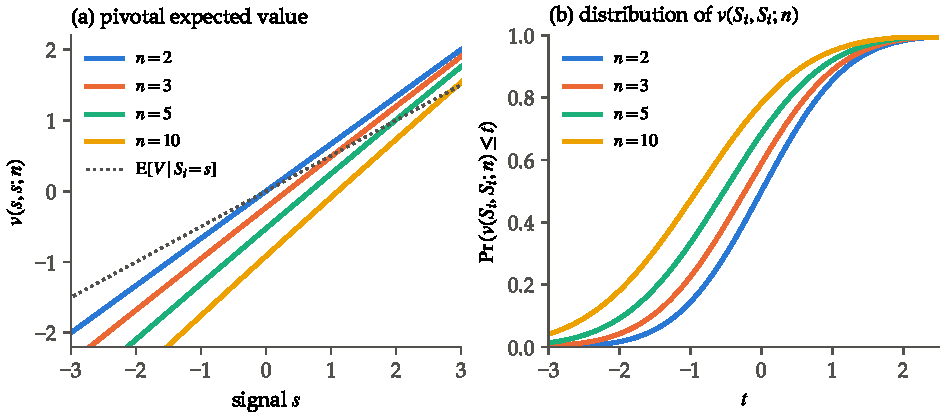
\includegraphics[width=\textwidth]{figures/ch15/cv_winners_curse.pdf}
  \caption{The winner's curse and the number of bidders in a Gaussian mineral rights model: $V_0\sim N(0,1)$
  and $S_i=V_0+e_i$ with independent $e_i\sim N(0,1)$. Panel (a): the pivotal expected value $v(s,s;n)$ falls
  with $n$ for every signal (\cref{lem:15-pivotal-n}). The dotted line is $\E[V_0\mid S_i=s]=\frac s2$, which
  does not depend on $n$. Panel (b): the distribution of $v(S_i,S_i;n)$, the object compared across $n$ in the
  test of \citet{HaileHongShum2003}. Under private values the four curves would coincide. Our computation by
  numerical integration, with no random numbers (script \texttt{cv\_winners\_curse.py}).}\label{fig:15-wc-n}
\end{figure}

\casehead{Endogenous participation} Exogenous variation in $n$ is a strong assumption. A binding reserve price
or a bid-preparation cost truncates the set of participating types. \citet{HaileHongShum2003} adjust for
truncation and compare the distributions on their common support \citep[Section~8.2]{AtheyHaile2007}.
Unobservables that move both participation and values are harder. If more valuable tracts attract more bidders,
that variation can mask the winner's curse. Unobserved heterogeneity also threatens identification of $F_{v,n}$
itself (\cref{sec:15-uh}). \citet{HaileHongShum2003} propose an instrumental approach that builds on
\cref{ass:15-cpv-uh}. Let the number of bidders be $n_t=\chi(Z_t,\omega_t)$, where $Z_t$ is observed and
$\omega_t$ is an unobserved index of the auction, the unobserved heterogeneity of \cref{sec:15-uh}. Assume
(i) $Z_t$ is independent of signals and values, and (ii) $\chi$ is weakly increasing in $Z_t$ and strictly
increasing in $\omega_t$. Strict monotonicity in $\omega_t$ makes $(n_t,Z_t)$ a sufficient statistic for
$\omega_t$. The pivotal expected value of a bidder whose signal $s$ leads to the bid $b$ is then identified
conditional on $(n_t,Z_t)$:
\begin{equation*}
  v(s,s;n,z)=b+\frac{\Pr\bigl(M_{it}\le b\mid B_{it}=b,\ Z_t=z,\ n_t=n\bigr)}{\frac{\partial}{\partial m}
  \Pr\bigl(M_{it}\le m\mid B_{it}=b,\ Z_t=z,\ n_t=n\bigr)\big|_{m=b}} .
\end{equation*}
Pooling pseudo-values across $n$ for each $z$, the distribution of pivotal values must be the same for all $z$
under private values. It shifts with $z$ under common values. In timber auctions they use the number of
sawmills and logging firms near a sale as the instrument \citep[Section~8.2]{AtheyHaile2007}. Strict
monotonicity in a scalar unobservable is the price of the approach. It also requires the unobservable to be
discrete, because $n_t$ is.

\casehead{Binding reserve prices} A reserve price offers a different test \citep{HendricksPinksePorter2003}.
With reserve $r$ in a symmetric first-price auction, a bidder participates if her signal exceeds the threshold
$s^\ast=\inf\{s:\E[V_i\mid S_i=s,\ Y_i\le s]\ge r\}$. The marginal participant bids $r$ and wins only when no rival
participates. Her pivotal expected value is $v(s^\ast,s^\ast;n)$. Under private values the two conditional
expectations coincide, so $v(s^\ast,s^\ast;n)=r$. Under common values
$\E[V_i\mid S_i=s^\ast,\ Y_i\le s^\ast]<\E[V_i\mid S_i=Y_i=s^\ast]$, so $v(s^\ast,s^\ast;n)>r$
\citep[eqs.~(8.7)--(8.8)]{AtheyHaile2007}. The inverse bid function at the bottom of the bid support,
$\lim_{b\downarrow r}\bigl[b+\frac{G_{M\mid B}(b\mid b)}{g_{M\mid B}(b\mid b)}\bigr]$, should equal $r$ under
private values and exceed it under common values. With private values the markdown vanishes at the reserve,
so rival bids are dense just above $r$ (compare \cref{thm:15-gpv-reserve}). With common values the markdown
stays positive, because even the marginal participant bids below her pivotal value. Bids just above $r$ are
then relatively sparse, an implication of the reserve price already noted by \citet{MilgromWeber1982}.
\citet{HillShneyerov2013} develop a formal test based on the tail of the bid distribution near the reserve.

\casehead{Evidence from timber, oil and procurement auctions} The tests have been applied in several
markets, and the answer depends on the market \citep[Sections~2.3, 3.2 and 4.1]{HortacsuPerrigne2021}. In
Forest Service first-price sales in the western half of the United States, the tests of
\citet{HaileHongShum2003} find no evidence of common values in scale sales. We report the results of the
2006 revision of that working paper, as summarized by \citet[pp.~93--94]{HortacsuPerrigne2021}. The evidence is
mixed in lump-sum sales, where the case for common values was stronger.
\citet{CompianiHaileSantAnna2020} extend the test to endogenous entry and unobserved heterogeneity and apply
it to Outer Continental Shelf leases (pp.~126--127). Private information is multiplicatively separable into a
function of observed and unobserved heterogeneity and an idiosyncratic base value. Bids then decompose into
the same function times a \emph{homogenized bid} that depends only on the number of bidders and the signal.
The number of bidders depends on observables and rises weakly with the unobservable. An instrument shifts
entry but not signals or values, and in the application it is the number of neighbor firms. Under private
values the joint distribution of signals and values does not depend on the number of bidders, while common
values order it by stochastic dominance. The authors conclude in favor of common values. Ignoring unobserved
heterogeneity would produce an ordering contrary to common values, a misspecification of the kind studied in
\cref{sec:15-uh}. For policy, the seller would not gain from limiting competition to soften the winner's
curse. A second-price auction, which exploits the linkage principle (\cref{prop:14-linkage}), would raise
revenue only slightly.

\citet{HongShum2002} quantify the winner's curse in procurement with a parametric model of affiliated values
(pp.~104--105). Under common values more bidders have two effects on bids. A competitive effect lowers them,
and a winner's-curse effect raises them, so bids can be U-shaped in the number of bidders. The model follows
the log-additive specification of Wilson, with multiplicative decompositions of costs and signals. The
relative standard deviations of the common component, the private component and the signal noise measure
how common the costs are. In New Jersey Department of Transportation auctions, highway work behaves like
common values, while bridge work and road paving mix private and common values. Allowing for unobserved
heterogeneity, road paving looks like independent private costs and highway work like affiliated private
values. For highway work, halving the number of bidders would lower the procurement cost by 15 percent. For
the other two kinds of work, more competition lowers the cost, so the competitive effect dominates.

\Cref{tab:15-cv-tests} collects the tests of this subsection. Each one replaces the unattainable goal of
identifying $F_{\bm S,\bm V}$ by a restriction that private values impose and common values violate.

\begin{table}[htbp]
\centering
\caption{Tests of private against common values}\label{tab:15-cv-tests}
\small
\begin{tabularx}{\textwidth}{@{}>{\raggedright\arraybackslash}p{2.6cm}>{\raggedright\arraybackslash}X>{\raggedright\arraybackslash}X>{\raggedright\arraybackslash}p{2.5cm}@{}}
\toprule
Format & Data and variation & Restriction under private values & Source \\
\midrule
Second-price or ascending & Price with $m$ bidders, upper bids with $n>m$. Exogenous $n$ & Recurrence
\eqref{eq:15-recurrence} holds (in means for ascending). Common values give dominance & \citet[Thm.~9]{AtheyHaile2002} \\
Second-price, asymmetric & Bids with $n$ bidders, prices with subsets of bidders & Recurrence for random
subsamples & \citet[Thm.~10]{AtheyHaile2002} \\
First-price & Top two bids with $n$ and $n-1$ bidders & Recurrence for identified $v(S,S;n)$ & \citet[Thm.~11]{AtheyHaile2002} \\
First-price & All bids, exogenous $n$ & $F_{v,n}$ invariant to $n$. It falls in $n$ under common values &
\citet{HaileHongShum2003} \\
First-price & All bids, instrument for $n$ & Pivotal values invariant to the instrument & \citet{HaileHongShum2003} \\
First-price & All bids, instrument for entry, unobserved heterogeneity & Joint law of signals and values invariant to $n$ & \citet{CompianiHaileSantAnna2020} \\
First-price & Binding reserve price & Inverse bid function equals $r$ at the bottom & \citet{HendricksPinksePorter2003} \\
First-price & All bids and ex post values & Overidentifying restriction \eqref{eq:15-hpp-test} & \citet{HendricksPinksePorter2003} \\
First-price, two bidders & Bids and identities & Quasi-symmetry rejects asymmetric pure common values & \citet{CampoPerrigneVuong2003} \\
\bottomrule
\end{tabularx}
\end{table}

\subsection{Interdependent costs: Somaini (2020)}\label{sec:15-cv-somaini}

\casehead{Question} Most empirical work picks one of two polar models. Under private costs there is no
winner's curse. Under pure common costs every bidder would incur the same cost, so the allocation cannot be
inefficient. Intermediate models had received little attention, largely because \citet{LaffontVuong1996}
showed that any bid distribution rationalized by interdependent costs is also rationalized by private costs.
\citet{Somaini2020} asks whether richer variation in competitive conditions restores identification in
procurement auctions. The variation comes from continuous bidder-specific cost shifters, such as each firm's
distance to the project. The test of \citet{HaileHongShum2003} uses discrete variation in $n$. Continuous
shifters vary competition in more directions.

\casehead{Primitives} A buyer procures a project by first-price (low-bid) sealed bid from $n$ risk-neutral
bidders, with no reserve price. Bidder $i$'s cost is $C_i$ and her private information is a scalar signal
$S_i$. Signals are normalized to have uniform marginals, so their joint distribution $F_{\bm S}$ is a copula.
Each bidder has a public cost shifter $w_i$, and $\bm w=(w_1,\dots,w_n)$. Somaini writes $x_i$ for $w_i$ and
conditions on auction characteristics throughout. Bidder $i$'s \emph{full-information cost} is
\begin{equation*}
  c_i(\bm s_{-i},s_i,w_i)=\E\left[C_i\mid \bm S=\bm s,\ \bm w\right].
\end{equation*}
For risk-neutral bidders, the payoff-relevant primitives are $F_{\bm S}$ and the functions $c_i$. They are
coarser than the joint distribution of costs and signals. They suffice for counterfactuals that change the rules,
the reserve price or subsidies \citep[Section~I]{Somaini2020}.

\begin{assumption}[{\citealp[Assumptions~A1--A3 and A7]{Somaini2020}}]\label{ass:15-somaini}
(A1) Signals are independent of cost shifters: $F_{\bm S\mid\bm w}=F_{\bm S}$. (A2) Signals are scalar, and
$F_{\bm S}$ has a continuously differentiable bounded density $f$. (A3) Rivals' shifters are excluded from a
bidder's full-information cost: $\E[C_i\mid\bm S,\bm w]=c_i(\bm S_{-i},S_i,w_i)$. (A7) For every $\bm w$, the
data are generated by repeated play of the same Bayes-Nash equilibrium in monotone pure strategies.
\end{assumption}

The model nests the standard cases. Private costs mean $c_i$ does not depend on $\bm s_{-i}$. Independent
private costs add independence of signals, and affiliated private costs allow affiliation. Pure common costs
mean $c_i=c_j$ for all $i,j$. Bidders may also be asymmetric in any way. Assumptions A1 and A3 define what makes
an observable a cost shifter. For distance, they rule out a firm having lower costs when a rival is nearby. They
also rule out a firm regarding a nearby rival's signal as more informative. Equilibria in monotone pure strategies
exist when signals are affiliated \citep{RenyZamir2004}. Somaini shows that without a binding reserve price they
are strictly increasing \citep[Proposition~1]{Somaini2020}.

\casehead{First-order condition} Let $s_j(b)=\beta_j^{-1}(b)$ be the signal at which rival $j$ bids $b$. A low
bid wins, so bidder $i$ wins with bid $b$ when $\bm S_{-i}\ge\bm s_{-i}(b)$ componentwise. Her expected
profit is
\begin{equation*}
  \Pi_i(b;s_i)=\int_{\bm\tau\ge\bm s_{-i}(b)}\bigl(b-c_i(\bm\tau,s_i,w_i)\bigr)f(\bm\tau\mid s_i)\,d\bm\tau .
\end{equation*}
Differentiating in $b$ gives one term from the margin $b$ and one boundary term for each rival:
\begin{multline*}
  \Pr\bigl(\bm S_{-i}\ge\bm s_{-i}(b)\mid s_i\bigr)
  -\sum_{j\ne i}s_j'(b)f\bigl(s_j(b)\mid s_i\bigr)\Pr\bigl(\bm S_{-ij}\ge\bm s_{-ij}(b)\mid s_i,s_j(b)\bigr)\\
  \times\Bigl[b-\E\bigl(C_i\mid s_i,\,s_j(b),\,\bm S_{-ij}\ge\bm s_{-ij}(b)\bigr)\Bigr]=0 .
\end{multline*}
Let $D_i(b)$ be the sum of the weights $s_j'(b)f(s_j(b)\mid s_i)\Pr(\bm S_{-ij}\ge\bm s_{-ij}(b)\mid s_i,s_j(b))$.
It equals the absolute derivative of the win probability in the bid. Let $\pi^{(i)}_j(b)$ be rival $j$'s weight
divided by $D_i(b)$. Rearranging,
\begin{equation}\label{eq:15-som-foc}
  b-\frac{\Pr\bigl(\bm S_{-i}\ge\bm s_{-i}(b)\mid s_i\bigr)}{D_i(b)}
  =\sum_{j\ne i}\pi^{(i)}_j(b)\,\E\Bigl(C_i\mid s_i,\ S_j=s_j(b),\ \bm S_{-ij}\ge\bm s_{-ij}(b),\ w_i\Bigr),
\end{equation}
equation (5) of \citet{Somaini2020}. The left side is marginal revenue, the bid minus a markup. The right side
is the expected cost conditional on the bid being \emph{pivotal}, that is, tying with at least one rival for the
lowest bid. The weight $\pi^{(i)}_j$ is the probability of tying with rival $j$ given a tie with at least one
rival.

\casehead{Identification} The argument has three steps. First, monotone strategies imply that the copula of bids
equals the copula of signals. With uniform signals, $s_i=H_{B_i\mid\bm w}(b_i)$, the marginal distribution of
$i$'s bid given $\bm w$. Hence $F_{\bm S}(\bm s)=H_{\bm B\mid\bm w}\bigl(Q_{B_1\mid\bm w}(s_1),\dots,Q_{B_n\mid\bm
w}(s_n)\bigr)$, where $Q$ denotes a quantile function \citep[Lemma~1 and Proposition~3]{Somaini2020}. By A1, the
bid copula must not vary with $\bm w$, a testable implication. Nonparticipation is recorded as an infinite bid.

Second, the left side of \eqref{eq:15-som-foc} is identified as in \eqref{eq:15-lpv-foc}, because conditioning on
the signal is conditioning on the bid. With $M_i=\min_{j\ne i}B_j$,
\begin{equation}\label{eq:15-som-xi}
  \xi_i(b_i,\bm w)=b_i-\frac{\Pr(M_i\ge b_i\mid B_i=b_i,\bm w)}{\bigl|\frac{\partial}{\partial m}\Pr(M_i\ge m\mid
  B_i=b_i,\bm w)\big|_{m=b_i}\bigr|} .
\end{equation}
The right side is the limit as $\varepsilon\downarrow0$ of $\E\bigl(C_i\mid S_i=s_i,\ \bm S_{-i}\in
L_\varepsilon(b_i,\bm w),\ w_i\bigr)$. Here $L_\varepsilon(b,\bm w)$ is the set of rival signals for which $i$ wins
with bid $b$ but loses with $b+\varepsilon$. It is the difference of two rectangles, each identified from the
marginal bid distributions.

Third, variation in rivals' shifters moves these sets. With two bidders the pivotal event is a single point, and
\eqref{eq:15-som-foc} becomes
\begin{equation}\label{eq:15-som-two}
  \xi_1(b_1,\bm w)=c_1\bigl(H_{B_2\mid\bm w}(b_1),\,H_{B_1\mid\bm w}(b_1),\,w_1\bigr),
\end{equation}
equation (8) of \citet{Somaini2020}. Holding $w_1$ fixed and varying $(w_2,b_1)$ evaluates $c_1(\cdot,\cdot,w_1)$
at different pairs of signals. A3 ensures that $w_2$ moves the evaluation point without shifting $c_1$ itself. The
rival's shifter works like an instrument for the rival's signal.

With three bidders the pivotal set is L-shaped (\cref{fig:15-som-L}). One bid gives one equation in two
unknowns, the expected costs conditional on tying with bidder 2 or with bidder 3. Different rival shifters
$\bm w'$ produce another L-shaped set stacked on the first, with $s_1$ and $w_1$ fixed. Under A1, the expected
cost over the union is a probability-weighted average with identified weights. Stacking ever finer L-shaped sets
covers the rectangle $\{S_2\ge s_2,\ S_3\ge s_3\}$. The limit identifies $\E(C_1\mid s_1,\ S_2\ge s_2,\ S_3\ge
s_3,\ w_1)$, the expected cost conditional on winning. Differentiating twice recovers the full-information cost:
\begin{multline}\label{eq:15-som-diff}
  \frac{\partial^2}{\partial s_2\,\partial s_3}\Bigl[\E\bigl(C_1\mid s_1,S_2\ge s_2,S_3\ge s_3,w_1\bigr)
  \Pr\bigl(S_2\ge s_2,S_3\ge s_3\mid s_1\bigr)\Bigr]\\
  =c_1(s_2,s_3,s_1,w_1)\,f_{S_2,S_3\mid S_1}(s_2,s_3),
\end{multline}
equation (10) of \citet{Somaini2020}. The two minus signs from differentiating the lower limits cancel.

\begin{figure}[htbp]
\centering
\begin{tikzpicture}[scale=5.2,>=Stealth]
  \fill[blue!8] (0.42,0.30) rectangle (1,1);
  \fill[blue!35] (0.42,0.30) -- (1,0.30) -- (1,0.36) -- (0.48,0.36) -- (0.48,1) -- (0.42,1) -- cycle;
  \fill[orange!45] (0.48,0.36) -- (1,0.36) -- (1,0.42) -- (0.54,0.42) -- (0.54,1) -- (0.48,1) -- cycle;
  \draw[thick] (0,0) rectangle (1,1);
  \draw (0.42,0.30) rectangle (1,1);
  \draw (0.48,0.36) rectangle (1,1);
  \draw (0.54,0.42) rectangle (1,1);
  \fill (0.42,0.30) circle (0.010);
  \fill (0.48,0.36) circle (0.010);
  \node[below left] at (0,0) {$0$};
  \node[below] at (1,0) {$1$};
  \node[left] at (0,1) {$1$};
  \node[below] at (0.5,-0.06) {rival signal $S_2$};
  \node[rotate=90] at (-0.1,0.5) {rival signal $S_3$};
  \node[font=\small] at (0.20,0.12) {$\bigl(s_2(b),s_3(b)\bigr)$};
  \draw[->] (0.24,0.16) -- (0.41,0.29);
  \node[font=\small] at (0.78,0.12) {$L_\varepsilon(b,\bm w)$};
  \draw[->] (0.78,0.16) -- (0.78,0.32);
  \node[font=\small,anchor=east] at (0.31,0.66) {$L_\varepsilon(t,\bm w')$};
  \draw[->] (0.32,0.66) -- (0.505,0.66);
  \node[font=\small,align=center] at (0.77,0.72) {win region\\ not yet\\ covered};
\end{tikzpicture}
\caption{Pivotal sets with three bidders in a procurement auction, drawn in the space of bidder 1's rivals'
signals. Bidder 1 wins with bid $b$ when both rival signals exceed the thresholds $s_2(b)$ and $s_3(b)$. The
blue L-shaped set $L_\varepsilon(b,\bm w)$ contains the rival signals for which bidder 1 wins with $b$ but loses
with $b+\varepsilon$. The first-order condition identifies the expected cost on this set. Different rival
shifters $\bm w'$ and a bid $t$ produce the stacked orange set $L_\varepsilon(t,\bm w')$, holding bidder 1's
signal and shifter fixed. Stacking such sets fills the light rectangle. Our drawing, after \citet[Figures~1--2]{Somaini2020}.}\label{fig:15-som-L}
\end{figure}

\begin{theorem}[{\citealp[Theorem~4]{Somaini2020}}]\label{thm:15-somaini}
Under \cref{ass:15-somaini}, the full-information cost $c_i(\bm s_{-i},s_i,w_i)$ is identified for all
$\bm s\ge\bm s^\ast$ if the observables exhibit sufficient variation and nonvanishing competition for bidder $i$
at $(\bm s^\ast,w_i)$.
\end{theorem}

Sufficient variation has a precise meaning \citep[Definition~1]{Somaini2020}. For every $\bm s\ge\bm s^\ast$
there must be rival shifters $\bm w_{-i}$ and a finite bid $b$ with $H_{B_j\mid\bm w}(b)=s_j$ for every bidder
$j$. The bid $b$ is then bidder $i$'s equilibrium bid at signal $s_i$. Nonvanishing competition bounds the number of L-shaped sets
needed, by requiring rivals to bid in any interval $[b,b']$ with nonvanishing probability (Definition~2).
Equilibrium observables of first-price auctions typically exhibit nonvanishing competition. A bounded set of
shifters suffices for signals bounded away from zero \citep[Propositions~5--6]{Somaini2020}. Identification at
extreme signals may need shifters with unbounded support.

Three limits deserve mention \citep[Section~III.C]{Somaini2020}. Binding reserve prices can reduce the variation
that shifters generate. Entry costs paid after learning signals are hard to distinguish from full-information
costs that rise sharply as rivals' signals approach the top. A random entry cost unobserved by the econometrician
violates A7, so \cref{thm:15-somaini} does not apply. Finally, the identified primitives cannot evaluate
counterfactuals in which bidders act after learning more, such as resale or subcontracting once costs are known.

\casehead{Setting and data} The Michigan Department of Transportation (MDOT) awards about 1,050 highway contracts
a year, worth about \$1.2 billion in total, by first-price sealed bid. On each monthly letting date, 150 to 200
firms bid on 50 to 70 contracts \citep[p.~3844]{Somaini2020}. Contracts are advertised at least 45 days ahead.
There is no formal reserve price, but the agency may reject all bids if the lowest exceeds 110 percent of the
engineer's estimate. From 2001 to 2010 the lowest bid exceeded that level in 11 percent of cases, and 15 percent
of these were rejected (p.~3845). The study focuses on hot-mixed asphalt paving. The mix must be compacted while
hot, above $135^\circ$C, so trucking time from a firm's plant matters for cost and quality. Distance from the plant
to the project is the cost shifter. Of 10,522 auctions from January 2001 to December 2010, 3,851 required asphalt
prequalification, and 1,925 had it as the only requirement. These form the sample (p.~3846).

In the sample the median engineer's estimate is \$633,000 and the median lowest bid \$586,000. Auctions have 3.04
participants on average. The median normalized winning bid, $\frac{\text{lowest bid}}{\text{estimate}}-1$, is
$-6.8$ percent. The second-lowest bid exceeds the lowest by 8.2 percent on average. The median participant is 38
km from the project and the median winner 22 km (Table~1). The average winning bid falls with the number of
participants, but the average bid does not (Table~2). Somaini reads this as evidence against the symmetric
independent private cost model with exogenous participation.

\casehead{Econometric model} Signals are mapped to standard normals, $\zeta_i=\Phi^{-1}(S_i)$, with
$\bm\zeta\sim N(0,\Sigma)$ and a factor structure $\Sigma=LL^\top+\Lambda$. Let $Z_t$ be auction characteristics.
The Gaussian information structure implies
\begin{equation}\label{eq:15-som-gauss}
  \E\bigl(C_i\mid\bm\zeta,Z_t,w_i\bigr)=\alpha_{ic}+Z_t\alpha_{i0}+\alpha_{i1}w_i
  +\alpha_{i2}\sum_{j\ne i}\tilde\sigma_{ij}\zeta_j+\nu_i\zeta_i,
\end{equation}
where $\tilde\sigma_{ij}$ is the $(i,j)$ element of $-\Sigma^{-1}$, nonnegative under affiliation
\citep[eq.~(11)]{Somaini2020}. Here $\Phi$ is the standard normal distribution function. One parameter per
bidder, $\alpha_{i2}$, measures interdependence. Private costs are $\alpha_{i2}=0$, interdependent costs are
$\alpha_{i2}>0$, and $\alpha_{i2}<0$ would falsify the model. Substituting \eqref{eq:15-som-gauss} into
\eqref{eq:15-som-foc} gives the estimating equation
\begin{equation}\label{eq:15-som-est}
  B_i=\alpha_{ic}+Z_t\alpha_{i0}+\alpha_{i1}W_i+\alpha_{i2}\,k_i(B_i,\bm W\mid H)+\iota_i(B_i,\bm W\mid H)+\nu_i\zeta_i,
\end{equation}
equation (12). The term $\iota_i$ is the markup from market power, the second term of \eqref{eq:15-som-xi}. The
term $\alpha_{i2}k_i$ is the markup from the winner's curse, where
\begin{equation*}
  k_i=\sum_{j\ne i}\tilde\sigma_{ij}\Bigl[\pi^{(i)}_j\zeta_j(b)+\sum_{k\ne i,j}\pi^{(i)}_k\,
  \E\bigl(\zeta_j\mid\zeta_k=\zeta_k(b),\ \bm\zeta_{-ik}\ge\bm\zeta_{-ik}(b)\bigr)\Bigr]
\end{equation*}
depends only on the bid distribution $H$. A bidder knows that she wins only when rivals have drawn high signals.

\casehead{Estimator and instruments} Let $\nu_{i\tau}$ be the $\tau$-th quantile of $\alpha_{ic}+\nu_i\zeta_i$.
Since signals are independent of shifters, \eqref{eq:15-som-est} implies the quantile moment
$\E[\indic(B_i-Z_t\alpha_{i0}-\alpha_{i1}W_i-\alpha_{i2}k_i-\iota_i-\nu_{i\tau}\le0)-\tau\mid\bm W]=0$.
Nonparticipation censors bids. Only signals below a participation cutoff yield finite bids, and the cutoff has
probability $\phi_i(\bm W\mid H)$. The moment conditional on participation replaces $\tau$ by
$\min\bigl(\frac{\tau}{\phi_i(\bm W\mid H)},1\bigr)$ \citep[eqs.~(13)--(14)]{Somaini2020}. The parameters are
estimated by instrumental variable quantile regression \citep{ChernozhukovHansen2006}. The instrument for $k_i$
is its projection on the bidder's own covariates and rivals' distances. Rivals' distances are excluded from own
cost by A3, and they move the pivotal sets and hence $k_i$. The first stage estimates the marginal bid
distributions with cubic B-splines in the project's latitude, longitude and the bid, and the copula by simulated
maximum likelihood. The markups $\iota_i$ and $k_i$ come from spline estimates of win and tie probabilities.
Standard errors come from 200 bootstrap samples of the 1,925 auctions (p.~3850).

\casehead{Results} The analysis covers 19 frequent bidders, with the remaining firms grouped as a fringe
bidder. The Akaike criterion selects two factors. The first factor creates correlations of 0.11 to 0.29 among one
group of firms and explains up to 20 percent of their signal variance. The second explains up to 25 percent for
another group (pp.~3854--3855). For bidder 1, the full-information cost at the 25th percentile of its own signal
and the median of rivals' signals is 73 percent of the engineer's estimate for projects within 10 km. The
interdependence coefficient $\alpha_{i2}$ is 0.500 (s.e.\ 0.190) for bidder 1, 0.350 (0.118) for bidder 2 and
$-0.025$ (0.092) for bidder 3 (Table~5). \Cref{tab:15-somaini-signals} reproduces the effects of own and rivals'
signals. A one standard deviation increase in bidder 1's own signal raises its full-information cost by 10
percentage points of the estimate. The same increase in a rival's signal raises it by 4 points on average and 7
at most (p.~3857). Rivals' signals matter, but less than one's own. Private costs are rejected for bidders 1 and
2. They cannot be rejected for bidders 3 and 9.

\begin{table}[htbp]
\centering
\caption{Effect of signals on full-information costs, Michigan highway procurement}\label{tab:15-somaini-signals}
\small
\begin{tabular}{@{}lcccccc@{}}
\toprule
 & \multicolumn{2}{c}{Own signal} & \multicolumn{2}{c}{Competitor (mean)} & \multicolumn{2}{c}{Competitor (maximum)} \\
\cmidrule(lr){2-3}\cmidrule(lr){4-5}\cmidrule(lr){6-7}
 & Coef. & S.e. & Coef. & S.e. & Coef. & S.e. \\
\midrule
Bidder 1 & 0.10*** & 0.02 & 0.04*** & 0.01 & 0.07*** & 0.02 \\
Bidder 2 & 0.09*** & 0.02 & 0.03*** & 0.01 & 0.06*** & 0.02 \\
Bidder 3 & 0.13*** & 0.05 & 0.00 & 0.00 & 0.00 & 0.01 \\
Bidder 4 & 0.59* & 0.32 & 0.00 & 1.15 & 0.00 & 3.95 \\
Bidder 5 & 0.13*** & 0.02 & 0.01*** & 0.00 & 0.02*** & 0.01 \\
Bidder 6 & 0.15 & 0.11 & 0.04* & 0.02 & 0.09** & 0.04 \\
Bidder 7 & 0.12*** & 0.04 & 0.03*** & 0.01 & 0.07*** & 0.02 \\
Bidder 8 & 0.32*** & 0.12 & 0.05 & 0.05 & 0.14 & 0.15 \\
Bidder 9 & 0.18*** & 0.04 & 0.01 & 0.03 & 0.02 & 0.10 \\
Bidder 10 & 0.10*** & 0.04 & 0.02*** & 0.00 & 0.05*** & 0.02 \\
Bidder 11 & 0.10*** & 0.03 & 0.03*** & 0.01 & 0.06*** & 0.02 \\
Bidder 12 & 0.07 & 0.06 & 0.03 & 0.04 & 0.06 & 0.10 \\
Bidder 13 & 0.09* & 0.05 & 0.02** & 0.01 & 0.04 & 0.03 \\
Bidder 14 & 0.25*** & 0.09 & 0.00 & 0.01 & 0.01 & 0.02 \\
Bidder 15 & 0.20*** & 0.05 & 0.00 & 0.01 & 0.00 & 0.02 \\
Bidder 16 & 0.07 & 0.08 & 0.02 & 0.02 & 0.05 & 0.06 \\
Bidder 17 & 0.12*** & 0.04 & 0.04 & 0.12 & 0.09 & 0.33 \\
Bidder 18 & 0.22* & 0.11 & 0.07 & 0.15 & 0.20 & 0.41 \\
Bidder 19 & 0.15 & 0.10 & 0.02** & 0.01 & 0.06** & 0.02 \\
\bottomrule
\end{tabular}

\smallskip
\begin{minipage}{0.92\textwidth}
\footnotesize \textit{Notes.} Effect of a one standard deviation increase in a bidder's own Gaussian signal, and in a
competitor's signal, on the bidder's full-information cost, as a fraction of the engineer's estimate. The
competitor effect depends on the competitor's identity, and the table reports its mean and maximum. Standard
errors from 200 bootstrap samples. * $p<0.1$, ** $p<0.05$, *** $p<0.01$. Source: \citet[Table~7]{Somaini2020}.
\end{minipage}
\end{table}

\casehead{Counterfactuals} Somaini simulates restricting participation to the $N$ bidders with the lowest median
cost in 250 randomly drawn auctions. Three models are compared: the estimated common-cost model (CC), an
affiliated private cost model that sets $\alpha_{i2}=0$ (APC), and an independent private cost model that also
sets $L=0$ (IPC). Inviting more bidders lowers procurement costs in all three models. Going from two to seven
invitees lowers costs by 5.48 percentage points under IPC, 5.00 under APC and 4.40 under CC (p.~3862). The bidder
with the lowest median cost bids more aggressively with more rivals under IPC and APC. Under CC it bids less
aggressively, because the winner's curse worsens. \Cref{tab:15-somaini-comp} decomposes the cost saving. The
competitive and sampling effects lower costs. Affiliation and the winner's curse raise them. The winner's curse is
strong enough to make the first invitee bid higher when competition grows, but not strong enough to make
restricting entry profitable for the buyer.

\begin{table}[htbp]
\centering
\caption{Decomposition of the effect of inviting more bidders on procurement costs}\label{tab:15-somaini-comp}
\small
\begin{tabular}{@{}lcccccccc@{}}
\toprule
Invitees & 3 vs.\ 2 & 4 vs.\ 2 & 5 vs.\ 2 & 6 vs.\ 2 & 7 vs.\ 2 & 8 vs.\ 2 & 9 vs.\ 2 & 10 vs.\ 2 \\
\midrule
Competitive & 1.98 & 2.52 & 2.71 & 2.79 & 2.92 & 2.95 & 2.97 & 2.97 \\
Affiliation & $-0.45$ & $-0.57$ & $-0.51$ & $-0.50$ & $-0.59$ & $-0.61$ & $-0.63$ & $-0.64$ \\
Winner's curse & $-1.52$ & $-2.21$ & $-3.06$ & $-3.37$ & $-3.65$ & $-3.84$ & $-3.95$ & $-3.96$ \\
Sampling & 2.83 & 3.88 & 4.91 & 5.38 & 5.71 & 5.95 & 6.08 & 6.10 \\
Total & 2.84 & 3.63 & 4.05 & 4.30 & 4.40 & 4.45 & 4.47 & 4.47 \\
\bottomrule
\end{tabular}

\smallskip
\begin{minipage}{0.95\textwidth}
\footnotesize \textit{Notes.} Cost savings relative to inviting two bidders, with 100 equal to average procurement cost
with two invitees. The competitive effect is the fall in the average bid of the first invitee under IPC. The
affiliation effect is the difference in that fall between APC and IPC, and the winner's curse effect the
difference between CC and APC. The sampling effect is the difference between the first invitee's bid reduction
and the fall in procurement cost under CC. Source: \citet[Table~8, top panel]{Somaini2020}.
\end{minipage}
\end{table}

Interdependence also affects reserve prices. It lowers the probability of awarding the contract by as much as
0.1 when the reserve is about 90 percent of the estimate (p.~3864). Suppose MDOT must set one reserve for all
contracts. With a willingness to pay of 100 percent of the estimate, the optimal reserve is 86 percent. With a
willingness to pay of 150 percent, it is 125 percent. These reserves succeed with probabilities 0.67 and 0.99 and yield surpluses
of 12 and 57 percent of the estimate. Auction-specific reserves would add less than 1 percent of the estimate
(p.~3867). The 110 percent rule is consistent with a willingness to pay above 140 percent of the estimate.

\casehead{Assessment} The paper gives the first nonparametric identification result for asymmetric
interdependent-cost auctions with dependent signals. Identification comes from continuous variation in
competitive conditions, which is richer than variation in the number of bidders. The estimates place Michigan paving between the polar
paradigms, much closer to private costs. The application relies on strong structure. The Gaussian form summarizes
interdependence by one parameter per bidder and makes costs additively separable in rivals' signals. Distance must
satisfy A1 and A3, which fails if a nearby rival's signal is more informative. Participation is handled through
censoring at a cutoff, and signals are scalar. Infrequent bidders are pooled into one fringe bidder. These restrictions
buy precision in a sample of 1,925 auctions.

\subsection{An auction with an informed bidder: Hendricks and Porter (1988)}\label{sec:15-cv-hp}

\casehead{Question} \citet{HendricksPorter1988} test the equilibrium predictions of a common value auction with
asymmetric information. The setting is the federal sale of drainage leases on the Outer Continental Shelf. A
drainage tract is adjacent to a tract on which oil or gas has been found. Firms owning adjacent tracts, the
\emph{neighbor} firms, learn about the drainage tract from their own drilling. Other firms rely on seismic
surveys and public information. The data include ex post production, so the authors can measure who earns
rents and test whether bidding accounts for the winner's curse.

\casehead{Theory} The model of \citet{Wilson1967} and \citet{EngelbrechtWiggansMilgromWeber1983} is developed in
\cref{prop:14-emw}. One informed bidder observes a private and a public signal and forms the estimate $H$ of
the common value. The uninformed bidders observe only the public signal. In equilibrium the informed bidder bids
$\E[H\mid H\le h]$ above a cutoff, bids the reserve price below it, and abstains below the reserve. The
uninformed bidders randomize so that the highest uninformed bid has the same distribution as the informed bid
above the reserve. \citet[pp.~870--871]{HendricksPorter1988} list seven predictions.
\begin{enumerate}[label=(\arabic*)]
  \item No neighbor bid is less frequent than no non-neighbor bid.
  \item The neighbor wins at least half of the tracts that receive a bid, by \eqref{eq:14-hp-winprob}.
  \item Non-neighbors earn zero expected profit. They lose on tracts where no neighbor bids and gain where one
  does.
  \item The neighbor earns an information rent.
  \item Without a cost difference between bidders, the informed bid and the highest uninformed bid have
  approximately the same distribution given public information.
  \item The neighbor's strategy does not depend on the number of non-neighbors.
  \item The neighbor's bid increases in the public signal when a higher signal is good news.
\end{enumerate}
Prediction (6) is convenient, because only participating non-neighbors are observed. Their number causes no
selection bias in the neighbor's bid equation.

\casehead{Setting and data} The sample covers federal tracts off Louisiana and Texas sold between 1959 and 1969
in 8 drainage sales, 144 tracts in all \citep[p.~871]{HendricksPorter1988}. It excludes 25 tracts on which the
high bid was rejected, for lack of data. The winning bid, the bonus, is paid at the sale. The government also
receives a royalty of one sixth of revenues. A reserve price of \$25 per acre applied on most drainage leases.
The government rejected the high bid on 7 percent of wildcat and 15 percent of drainage tracts. The authors
compute ex post discounted revenues and costs from production through 1980, real wellhead prices and drilling cost
surveys, discounting at 5 percent a year. \Cref{tab:14-hp-table1} summarizes the sample. Drainage tracts had an
average winning bid of \$5.76 million, net profit of \$4.63 million and value of \$13.51 million, with 2.73 bidders
on average. The government captured 66 percent of the value of drainage tracts against 77 percent for wildcat
tracts (p.~866).

Of the 144 drainage tracts, 114 were adjacent to previously leased federal tracts, and these form the sample.
Neighbor firms are the owners of adjacent federal tracts. Of the 114 tracts, 40 had one neighbor firm and 74 had
more (their Figure~1). Yet only 16 of the 74 received more than one neighbor bid (p.~872). The authors therefore
assume that neighbor firms coordinate and submit at most one serious bid. Joint bidding was legal, and neighbors
may already have formed a joint venture to manage production from the common pool.
The empirical analogues are the largest neighbor bid $B_I$ and the largest non-neighbor bid $B_U$, each set to the
reserve price when no such bid is made. The numbers of neighbor and non-neighbor bids are $N_I$ and $N_U$. The ex
post gross profitability of the tract, $\pi_t$, proxies the neighbor's private information. The public
information is the number of neighbor tracts $N^{\mathrm{tr}}$, the ex post gross profit of the adjacent tract
$V^{\mathrm{adj}}$, and acreage (their Table~2).

\casehead{Estimating equations} For tract $t$ and bidder type $i\in\{I,U\}$, let
\begin{equation*}
  Y_{it}=W_{it}\bm\theta_i+\varepsilon_{it},\qquad
  \ln\frac{B_{it}}{r_t}=\begin{cases}Y_{it}&\text{if }Y_{it}\ge0,\\ 0&\text{otherwise,}\end{cases}
\end{equation*}
where $r_t$ is the reserve price and $W_{it}$ a row of regressors. The errors $(\varepsilon_{It},\varepsilon_{Ut})$
are bivariate normal with variances $\sigma_I^2$ and $\sigma_U^2$, covariance $\sigma_{IU}$ and correlation
$\rho_{IU}$. Bids are lognormal and censored at the reserve. Only tracts with at least one bid are observed. Tracts
fall into three sets: $\Omega_{++}$ with bids of both types, $\Omega_{+0}$ with only neighbor bids, and
$\Omega_{0+}$ with only non-neighbor bids. Let $Z(a,c;\rho)$ be the probability under a standard bivariate normal
with correlation $\rho$ that both components fall below $a$ and $c$, the probability of no bid. The log-likelihood
is $\sum_{\Omega_{++}}l_{1t}+\sum_{\Omega_{+0}}l_{2t}+\sum_{\Omega_{0+}}l_{3t}$, with
\begin{align*}
  l_{1t}&=-\ln(2\pi)-\frac12\ln|\Sigma|-\frac12\,\bm\varepsilon_t^\top\Sigma^{-1}\bm\varepsilon_t-\ln\left[1-Z\left(-\frac{W_{Ut}\bm\theta_U}{\sigma_U},-\frac{W_{It}\bm\theta_I}{\sigma_I};\rho_{IU}\right)\right],\\
  l_{2t}&=\ln\Phi\left(\frac{-W_{Ut}\bm\theta_U-\frac{\sigma_{IU}}{\sigma_I^2}\varepsilon_{It}}{\sqrt{\sigma_U^2-\frac{\sigma_{IU}^2}{\sigma_I^2}}}\right)
  -\ln\sigma_I+\ln\phi\left(\frac{\varepsilon_{It}}{\sigma_I}\right)-\ln\bigl[1-Z(\cdot)\bigr],
\end{align*}
and $l_{3t}$ symmetric to $l_{2t}$ \citep[p.~873]{HendricksPorter1988}. Here $\Phi$ and $\phi$ are the standard
normal distribution function and density. In $l_{2t}$ the first term is the probability that the non-neighbor
latent bid is negative given the neighbor's residual. The next two terms are the density of the neighbor bid. The
last term in each contribution conditions on at least one bid, which corrects for sample selection.

\casehead{Participation and returns} No neighbor bid was made on 19 tracts and no non-neighbor bid on 35. So at
least one neighbor bid on 83 percent of tracts and at least one non-neighbor on 68 percent (p.~874), as
prediction (1) requires.
\Cref{tab:15-hp} reproduces the returns by winner type. The neighbor won 59 of the 114 tracts, 52 percent, as
prediction (2) requires. It won 62 percent of the 95 tracts it bid on, the figure the authors report (p.~874). Its share of tract value was about 44 percent, against an average firm share of 23
percent on wildcat tracts (prediction 4). Non-neighbor winners earned about zero on average, $-0.42$ million.
They lost on tracts with no neighbor bid and gained on tracts with one, as prediction (3) requires. Neighbors
appear able to identify the tracts likely to contain oil.

\begin{table}[htbp]
\centering
\caption{Tracts won by neighbor and non-neighbor firms, OCS drainage sales 1959--1969}\label{tab:15-hp}
\small
\begin{tabular}{@{}lccccc@{}}
\toprule
\multicolumn{6}{@{}l}{\emph{Panel A. Wins by type of firm (Table 3)}}\\
 & \multicolumn{2}{c}{Neighbor wins} & \multicolumn{3}{c}{Non-neighbor wins} \\
\cmidrule(lr){2-3}\cmidrule(lr){4-6}
 & A & Total & B & C & Total \\
\midrule
Number of tracts & 35 & 59 & 19 & 36 & 55 \\
Tracts drilled & 23 & 47 & 18 & 33 & 51 \\
Productive tracts & 16 & 36 & 12 & 19 & 31 \\
Average winning bid & 3.28 & 6.04 & 2.15 & 6.30 & 4.87 \\
 & (0.56) & (2.00) & (0.67) & (1.31) & (0.92) \\
Average gross profits & 10.05 & 12.75 & $-0.54$ & 7.08 & 4.45 \\
 & (3.91) & (3.21) & (0.47) & (2.95) & (1.99) \\
Average net profits & 6.76 & 6.71 & $-2.69$ & 0.78 & $-0.42$ \\
 & (3.02) & (2.69) & (0.86) & (2.64) & (1.76) \\
\midrule
\multicolumn{6}{@{}l}{\emph{Panel B. Single and multiple neighbor tracts (Table 4)}}\\
 & Single & \multicolumn{3}{c}{Multiple neighbors, by neighbor bids} & \\
\cmidrule(lr){3-5}
 & neighbor & 1 & $\ge2$ & Total & \\
\midrule
Number of tracts & 40 & 48 & 15 & 74 & \\
Tracts with no neighbor bid & 8 & & & 11 & \\
Neighbor wins & 19 & 29 & 11 & 40 & \\
Neighbor's average winning bid & 4.795 & 2.615 & 17.193 & 6.624 & \\
 & (1.444) & (0.697) & (9.953) & (2.885) & \\
Neighbor's average gross profits & 13.601 & 4.670 & 32.597 & 12.350 & \\
 & (5.608) & (2.148) & (11.506) & (3.965) & \\
Neighbor's average net profits & 8.806 & 2.055 & 15.404 & 5.725 & \\
 & (4.762) & (1.690) & (10.963) & (3.297) & \\
\bottomrule
\end{tabular}

\smallskip
\begin{minipage}{0.92\textwidth}
\footnotesize \textit{Notes.} Millions of 1972 dollars. Standard deviations of the sample means in parentheses. In Panel
A, column A is tracts with no non-neighbor bid, column B tracts with no neighbor bid, and column C tracts on which
a neighbor bid but a non-neighbor won. Gross profits exclude the bonus, and net profits deduct it. The authors give 17
(p.~867), 16 (p.~872) and 15 (Table~4) as the number of tracts with more than one neighbor bid. Panel B reproduces
Table~4. Source: \citet[Tables~3 and~4]{HendricksPorter1988}.
\end{minipage}
\end{table}

The model also predicts a mass point of neighbor bids at the reserve price, from informed types between the
reserve and the cutoff. The authors find none. They suggest that firms feared the government would reject
reserve-price bids, as it did on 25 drainage tracts. The reserve also explains why non-neighbors drilled tracts
on which no neighbor bid. Drilling is rational if expected net profit given no neighbor bid is below the reserve
but positive once the bid is sunk. Panel B checks the coordination assumption. On single and multiple neighbor
tracts alike, the neighbor won about half of the tracts. Net profits on multiple neighbor tracts are not
significantly lower, so competition among neighbors did not dissipate rents. Valuable multiple neighbor tracts
attracted more than one neighbor bid and earned higher net profits. The authors suggest ``shadow'' bids
submitted to make bidding look competitive to the government (p.~875).

\casehead{Information structure} Regressions of $\pi_t$ on bids and participation test whether non-neighbors
have payoff-relevant private information (their Table~5). With neighbor variables and public information, the
$R^2$ is 0.640. Adding non-neighbor variables raises it to 0.699. Non-neighbor variables and public information
alone give 0.154. The neighbor bid enters with coefficient 3.55 (t-statistic 3.90) and its square with $-0.023$
($-2.57$). The $F$-statistic for the six non-neighbor variables is 3.22 with $(6,98)$ degrees of freedom. The
authors compare it with 3.71 as the 5 percent point and do not reject. They add that most of the non-neighbor
explanatory power comes from the interaction with the neighbor bid. By standard tables the 5 percent point of
$F(6,98)$ is about 2.19, so the statistic would reject at conventional levels (our calculation).

\casehead{Bid distributions} Prediction (5) concerns the joint distribution of $(B_I,B_U)$ given public
information. In the unrestricted bivariate model the two equations have similar coefficients and residual
standard deviations, 2.02 and 2.66. Equal coefficients are not rejected: the likelihood ratio statistic is 10.58,
below 11.07, the 5 percent point of $\chi^2(5)$. The residual correlation is 0.10 (t-statistic 0.94), so no omitted
public variable appears to drive both bids (their Table~6). Adding tract profitability changes the picture. The
coefficient on $\pi_t$ is 0.091 (t-statistic 4.30) in the neighbor equation and 0.028 (0.79) in the non-neighbor
equation. Equal coefficients are now rejected at 1 percent, with statistic 19.84 (their Table~7). Non-neighbors
appear to have no information correlated with profitability beyond the public variables. Their bids are
``noisier,'' with residual standard deviation 2.62 against 1.60 for neighbors. The informed bid rises with $\pi_t$
and with $V^{\mathrm{adj}}$ and does not depend on $N_U$ (prediction 6). The highest non-neighbor bid rises with
$N_U$, as an order statistic should. Where $N_U$ is excluded, it falls with the number of neighbor tracts
(their Table~8).

\casehead{A competitive alternative} Section IV of the paper estimates a model in which neighbors bid
independently, each with a private signal. The likelihood treats each neighbor's bid and the highest non-neighbor
bid as censored normal latent variables \citep[p.~880]{HendricksPorter1988}. Two results contradict competitive
bidding (their Table~9). First, each neighbor's bid falls with the number of neighbor firms, with coefficient
$-0.758$ (t-statistic $-3.96$). For lognormal signals the competitive bid should first rise with the number of
bidders. Citing \citet{Smiley1979}, the authors place the turning point at four bidders or more in their data
\citep[p.~880]{HendricksPorter1988}. Only ten tracts had four or more neighbor firms. Phantom bids, below the serious bid, are consistent with the pattern. Second, the number of
neighbor firms lowers the highest non-neighbor bid by less than it lowers neighbor bids. Under competition among
neighbors the less informed non-neighbors should react more, because their winner's curse worsens more.

\casehead{Interpretation, critiques and contribution} The evidence supports the informed-bidder model with
coordinated neighbors. Neighbors shade their bids well below their estimates and earn high returns. Non-neighbors
bid cautiously, avoid the winner's curse and break even on average. The analysis has limits. Bidders are risk
neutral, tracts are analyzed one at a time, and coordination among neighbors is assumed. The proxy for private
information is ex post profitability, which measures the neighbor's estimate with error. The censored lognormal
model is a statistical description of bids and is not derived from the equilibrium. The sample has only 114
tracts. The missing mass point at the reserve contradicts the model, and \citet{HendricksPorterWilson1994}
later model a random reservation price for that reason. In their model the reservation price is correlated
with the tract value, and values are affiliated. Uninformed bidders are then less likely to participate and,
when they do, tend to bid high, while informed bidders tend to bid low. The informed bid distribution
stochastically dominates the uninformed one within the support of the reservation price and coincides with it
above. The data support these predictions \citep[p.~125]{HortacsuPerrigne2021}.

The paper sits in a sequence of studies of the same leases \citep[pp.~124--125]{HortacsuPerrigne2021}. It
built on the comparison of wildcat and drainage tracts by \citet{HendricksPorterBoudreau1987}. Bids, profits
and net profits per acre are much larger on drainage tracts. The highest bid and the profit per acre are
positively correlated on drainage tracts and negatively on wildcat tracts. Most large firms would have earned
more by bidding less, a sign that they did not fully correct for the winner's curse.
\citet{HendricksPorterSpady1989} then focus on rejections. The government rejects the highest bid on 18
percent of drainage tracts and 9 percent of wildcat tracts, and rejected drainage bids are larger. They also
note that neighbor firms rarely compete, although a drainage tract can have up to eight neighbors. The
paper's lasting contribution is to show that ex post values let the econometrician see adverse selection. It
confirmed subtle equilibrium predictions in a field setting and led to the tests of
\citet{HendricksPinksePorter2003} based on \eqref{eq:15-hpp-test}.
